% 論文導讀：M. Klazar, "The transcendence of e via formal power series"
% 讀者：高中生。超出高中數學範圍的知識在第一部分先行說明。
%
% 編譯：scripts/compile.sh guide/transcendence-e-guide.tex
%       -> build/transcendence-e-guide.pdf
%
% 內文分章放在 parts/ 之下，由本檔 \input。
\documentclass[11pt, a4paper]{article}

\usepackage[a4paper, top=2.4cm, bottom=2.6cm, left=2.2cm, right=2.2cm]{geometry}
\usepackage{contex-cjk}   % 中文 + 拉丁字型與語言設定（環境提供）
\usepackage{contex-stem}  % amsmath, amssymb, mathtools, booktabs, siunitx, tikz ...

\usepackage{amsthm}
\usepackage{pgfplots}
\pgfplotsset{compat=1.18}
\usepgfplotslibrary{fillbetween}
\usetikzlibrary{matrix, shapes.geometric, fit, backgrounds, shadows}
\usepackage[most]{tcolorbox}
\usepackage[unicode, colorlinks, linkcolor=blue!55!black, citecolor=green!40!black,
            urlcolor=blue!55!black]{hyperref}
\pdfstringdefDisableCommands{\def\e{e}\def\Exp{Exp}\def\N{N}\def\Z{Z}\def\Q{Q}\def\R{R}\def\C{C}\def\dd{ d}}

% ---------- 版面 ----------
\renewcommand{\baselinestretch}{1.28}
\setlength{\parindent}{2em}
\setlength{\parskip}{0.35em}
\setcounter{tocdepth}{2}
\setcounter{secnumdepth}{2}

% ---------- 記號 ----------
\newcommand{\N}{\mathbb{N}}
\newcommand{\Z}{\mathbb{Z}}
\newcommand{\Q}{\mathbb{Q}}
\newcommand{\R}{\mathbb{R}}
\newcommand{\C}{\mathbb{C}}
\newcommand{\e}{\mathrm{e}}
\newcommand{\dd}{\,\mathrm{d}}
\newcommand{\Exp}{\mathrm{Exp}}
\newcommand{\coef}[1]{[x^{#1}]\,}
\DeclareMathOperator{\ord}{ord}

% ---------- 定理環境 ----------
\theoremstyle{definition}
\newtheorem{defn}{定義}[section]
\newtheorem{thm}[defn]{定理}
\newtheorem{prop}[defn]{命題}
\newtheorem{lem}[defn]{引理}
\newtheorem{exmp}[defn]{例子}
\newtheorem{exer}[defn]{練習}
\theoremstyle{remark}
\newtheorem*{rem}{註}
\newenvironment{pf}{\begin{proof}[證明]}{\end{proof}}

% ---------- 彩色方框 ----------
\newtcolorbox{prereq}[1]{%
  enhanced, breakable, colback=blue!4, colframe=blue!50!black,
  fonttitle=\bfseries, title={先備知識：#1}, left=1.2em, right=1em,
  boxrule=0.6pt, arc=2pt}
\newtcolorbox{keyidea}[1][關鍵想法]{%
  enhanced, breakable, colback=orange!6, colframe=orange!70!black,
  fonttitle=\bfseries, title={#1}, left=1.2em, right=1em, boxrule=0.6pt, arc=2pt}
\newtcolorbox{paperbox}[1][論文原文對照]{%
  enhanced, breakable, colback=gray!6, colframe=gray!55!black,
  fonttitle=\bfseries, title={#1}, left=1.2em, right=1em, boxrule=0.6pt, arc=2pt}
\newtcolorbox{warnbox}[1][小心]{%
  enhanced, breakable, colback=red!4, colframe=red!60!black,
  fonttitle=\bfseries, title={#1}, left=1.2em, right=1em, boxrule=0.6pt, arc=2pt}

% ---------- 圖的共用樣式 ----------
\tikzset{
  box/.style={draw, rounded corners=3pt, align=center, inner sep=6pt, minimum height=2.2em,
              fill=white, drop shadow={opacity=0.15}},
  lbl/.style={font=\small},
  arr/.style={-{Stealth[length=2.2mm]}, thick},
}
\pgfplotsset{every axis/.append style={font=\small, axis lines=middle,
             xlabel style={at={(ticklabel* cs:1.02)}, anchor=west},
             ylabel style={at={(ticklabel* cs:1.02)}, anchor=south}}}

\title{\textbf{「用形式冪級數證明 $\e$ 是超越數」論文導讀}\\[0.6em]
  \large 讀 M.~Klazar, \emph{The transcendence of $\e$ via formal power series}（arXiv:2601.01019）\\[0.3em]
  \normalsize 寫給高中生的版本}
\author{導讀撰寫：Claude}
\date{\today}

\begin{document}
\maketitle

\begin{abstract}
\noindent
這份導讀陪你讀一篇數學論文。論文只有十幾頁，卻把三個證明「$\e$ 是超越數」的方法放在一起比較：
希爾伯特（Hilbert）1893 年的古典分析證明、Beukers--Bézivin--Robba 在 1990 年用形式冪級數
（formal power series，以下簡稱 FPS）給出的證明，以及作者 Klazar 把希爾伯特證明「翻譯」成
FPS 語言的新證明。論文的真正主題不是「$\e$ 是超越數」這個事實（它早在 1873 年就被 Hermite
證明），而是一個基礎論的問題：\emph{能不能不用「不可數集合」就證明它？}
第一部分先把超出高中數學的知識補齊：代數數與超越數、$\e$ 的級數、階乘的成長速度、
廣義積分與歐拉的恆等式、形式冪級數與極點、可數與不可數。第二到第四部分依序走過論文的三節，
每一節都附上圖解。最後有習題與延伸閱讀。
\end{abstract}

\tableofcontents
\clearpage

\section*{導讀的使用方式}
\addcontentsline{toc}{section}{導讀的使用方式}

\subsection*{這篇論文在說什麼？}

論文標題是 \emph{The transcendence of $\e$ via formal power series}，作者 Martin Klazar
（布拉格查理大學），預印本編號 arXiv:2601.01019 [math.NT]（2026 年 1 月提交，同年 5 月修訂至第 8 版）。「$\e$ 的超越性」指的是：$\e=2.71828\ldots$ 這個數\emph{不是}任何一個
整數係數多項式方程的根。換句話說，不論你取多少個整數 $a_0,a_1,\ldots,a_n$（不全為 $0$），
\[
  a_0+a_1\e+a_2\e^2+\cdots+a_n\e^n\neq 0\,.
\]
這個事實在 1873 年由 Hermite 證明，1893 年希爾伯特給了一個精簡的版本。論文做了三件事：
\begin{enumerate}
  \item \textbf{第一節}：複述希爾伯特的證明，然後提出問題：這個證明用到「函數」
        $F(x)=p(x)\e^{-x}$，而一個定義在 $[0,+\infty)$ 上的實函數，看成「所有點對 $(x,F(x))$
        的集合」，是\emph{不可數}的集合。能不能把證明改寫成只用\emph{可數}的物件？
  \item \textbf{第二節}：介紹 Beukers、Bézivin 與 Robba 在 1990 年的證明，它只用
        「形式冪級數」（一種「寫不完的多項式」），而形式冪級數就是一串係數，是可數的物件。
        他們證明的是更一般的 Lindemann--Weierstrass 定理；論文把它\emph{特殊化}到 $\e$ 的情形，
        讓邏輯結構看得更清楚。
  \item \textbf{第三節}：作者自己的證明。把希爾伯特證明裡每一個「分析」步驟
        （代入、平移、積分、取極限）都翻譯成對係數序列的操作，於是同一個證明就不再需要
        不可數集合了。
\end{enumerate}

\subsection*{為什麼值得高中生讀？}

因為它同時示範了三件在課本裡很少見到的事：
\begin{itemize}
  \item \textbf{反證法可以「量化」}：證明的核心招數是「造出一個非零整數，卻又證明它的絕對值小於 $1$」。
        這個招數高中生完全可以掌握（我們會先用它證明 $\e$ 是無理數）。
  \item \textbf{同一個定理可以有完全不同的證明思路}：希爾伯特靠的是積分；
        Beukers 等人靠的是「有理函數的極點」；Klazar 則靠「把分析翻譯成代數」。
  \item \textbf{數學家會在意「證明用了哪些工具」}：這篇論文真正關心的是基礎論的潔癖：
        \emph{同樣的結論，能不能用更少、更「小」的集合得到？}
\end{itemize}

\subsection*{怎麼讀這份導讀}

\begin{itemize}
  \item 第一部分是先備知識。每個藍色方框「先備知識」都是高中課綱之外、但論文會用到的概念。
        如果你已經學過微積分（例如數學甲的多項式微積分），第 \ref{sec:calc} 節可以快速掃過，
        但請務必看「廣義積分」與「歐拉恆等式」兩段。
  \item 橘色方框「關鍵想法」是每個證明的靈魂，先讀它，再看細節。
  \item 灰色方框「論文原文對照」告訴你導讀的哪一段對應論文的哪一個命題，方便你對照原文。
  \item 紅色方框「小心」提醒常見的誤解。
  \item 本文用 $\N=\{1,2,3,\ldots\}$、$\N_0=\{0,1,2,\ldots\}$、$\Z$（整數）、$\Q$（有理數）、
        $\R$（實數）、$\C$（複數），與論文一致。$n!=1\cdot2\cdots n$ 是階乘，$0!=1$。
        $\binom{n}{k}$ 是高中的組合數 $C^n_k$。
\end{itemize}

\begin{figure}[htbp]
\centering
\begin{tikzpicture}[node distance=0.8cm and 1.0cm, font=\small]
  \node[box, fill=blue!6, text width=5.2cm] (s1) {\textbf{第一節}\\ 希爾伯特的分析證明\\
    {\footnotesize 積分 $\int_0^{+\infty}p_r(x)\e^{-x}\dd x$，拆成「小量 $A_r$」與「$r!$ 的倍數 $B_r$」}};
  \node[box, fill=blue!6, text width=5.2cm, right=of s1] (q) {\textbf{提問}\\ 證明用了不可數集合（函數 $F=p\e^{-x}$）\\ 能否只用可數物件？};
  \node[box, fill=orange!8, text width=5.2cm, below=of s1] (s3)
    {\textbf{第三節}\\ Klazar：希爾伯特證明的 FPS 版\\
    {\footnotesize 定義「半形式」的平移、牛頓積分、廣義積分，逐條證明它們和分析裡的性質一樣}};
  \node[box, fill=orange!8, text width=5.2cm, below=of q] (s2)
    {\textbf{第二節}\\ Beukers--Bézivin--Robba\\
    {\footnotesize 若 $\e$ 是代數數，則某個 FPS $V(x)$ 既是有理的，又滿足一個微分方程，而極點的階數會互相矛盾}};
  \node[box, fill=green!8, text width=6cm, anchor=north] (end) at ($(s3.south)!0.5!(s2.south)+(0,-0.8cm)$)
    {\textbf{結論}\\ 兩個不使用不可數集合的證明都得到：$\e$ 是超越數};
  \draw[arr] (s1) -- (q);
  \draw[arr] (q) -- (s2);
  \draw[arr] (q) -- (s3);
  \draw[arr, dashed, gray] (s1) -- node[lbl, left, text=gray!60!black]{翻譯} (s3);
  \draw[arr] (s2) -- (end);
  \draw[arr] (s3) -- (end);
\end{tikzpicture}

\caption{論文的地圖。第一節提出問題，第二、三節各給一個回答。}
\label{fig:map}
\end{figure}

\clearpage
\part{先備知識：高中課本沒教的部分}
\section{代數數、超越數，與 $\e$ 這個數}\label{sec:numbers}

\subsection{代數數與超越數}

\begin{prereq}{代數數（algebraic number）與超越數（transcendental number）}
一個複數 $\alpha$ 叫做\textbf{代數數}，如果存在一個\emph{不是零多項式}的整數係數多項式
$f(x)=a_0+a_1x+\cdots+a_nx^n$（$a_i\in\Z$），使得 $f(\alpha)=0$。
不是代數數的複數叫做\textbf{超越數}。
\end{prereq}

\begin{exmp}
\begin{itemize}
  \item 每個有理數都是代數數：$\tfrac{3}{7}$ 是 $7x-3=0$ 的根。
  \item $\sqrt2$ 是代數數：它是 $x^2-2=0$ 的根。$\sqrt[3]{5}$ 是 $x^3-5=0$ 的根。
  \item 虛數單位 $i$ 是代數數：$x^2+1=0$。黃金比例 $\tfrac{1+\sqrt5}{2}$ 是 $x^2-x-1=0$ 的根。
  \item $\sqrt2+\sqrt3$ 也是代數數。令 $x=\sqrt2+\sqrt3$，則 $x^2=5+2\sqrt6$，
        $(x^2-5)^2=24$，所以 $x$ 是 $x^4-10x^2+1=0$ 的根。
\end{itemize}
\end{exmp}

所以「$\e$ 是超越數」的意思，就是導讀開頭寫的那句話：不論整數 $a_0,\ldots,a_n$（不全為零）怎麼取，都有 $a_0+a_1\e+\cdots+a_n\e^n\neq0$。
論文的每一個證明都從「假設它等於 $0$」出發，推出矛盾，這就是高中學過的\textbf{反證法}。

\begin{figure}[htbp]
\centering
\begin{tikzpicture}[font=\small]
  \draw[fill=gray!8, rounded corners=8pt] (-5.6,-2.3) rectangle (5.6,2.3);
  \node[anchor=north west] at (-5.5,2.25) {複數 $\C$};
  \draw[fill=orange!15, rounded corners=8pt] (-5.2,-1.75) rectangle (1.9,1.75);
  \node[anchor=north west] at (-5.1,1.7) {代數數};
  \draw[fill=blue!10, rounded corners=6pt] (-4.8,-1.2) rectangle (-0.6,1.2);
  \node[anchor=north west] at (-4.7,1.15) {有理數 $\Q$};
  \draw[fill=blue!22, rounded corners=5pt] (-4.4,-0.7) rectangle (-1.4,0.7);
  \node at (-2.9,0.15) {整數 $\Z$};
  \node at (-2.9,-0.35) {\footnotesize $0,\pm1,\pm2,\ldots$};
  \node at (0.6,0.6) {$\sqrt2$};
  \node at (1.2,-0.2) {$i$};
  \node at (0.4,-0.9) {$\sqrt2+\sqrt3$};
  \node[text=red!70!black] at (3.8,1.1) {$\e$};
  \node[text=red!70!black] at (3.2,0.1) {$\pi$};
  \node[text=red!70!black] at (4.3,-0.6) {$\e^{\pi}$};
  \node[text=red!70!black] at (3.4,-1.4) {$2^{\sqrt2}$};
  \node[anchor=south east, text=red!70!black] at (5.5,-2.25) {超越數（代數數以外的全部）};
\end{tikzpicture}
\caption{數的分類。代數數包含所有有理數和所有「根號式」。超越數是其餘的複數；
圖中列出的四個都已被證明是超越數（$\e^\pi$ 與 $2^{\sqrt2}$ 由 Gelfond--Schneider 定理，1934）。}
\label{fig:classes}
\end{figure}

\paragraph{一點歷史。}
1844 年 Liouville 造出第一個超越數（$\sum_{k\ge1}10^{-k!}=0.110001000\ldots$）。
1873 年 Hermite 證明 $\e$ 是超越數，這是第一個「自然出現的」超越數。
1882 年 Lindemann 用同樣的方法證明 $\pi$ 是超越數，順便解決了兩千年來的「化圓為方」問題。
1893 年希爾伯特把兩個證明精簡成幾頁，論文第一節複述的就是這個版本。
另外，1874 年 Cantor 證明超越數「多到數不完」，但他的證明不會告訴你任何一個具體的超越數是誰；
這和本文第 \ref{sec:countable} 節的「可數／不可數」有關。

\subsection{$\e$ 是什麼？指數級數}

高中課本把 $\e$ 當成「自然對數的底」，大約是 $2.71828$。本篇論文則把 $\e$ 和指數函數
看成一個\emph{無窮級數}，這是接下來一切的起點。

\begin{prereq}{$\e$ 與 $\e^x$ 的級數定義}
\[
  \e:=\sum_{n\ge0}\frac{1}{n!}=1+1+\frac12+\frac16+\frac1{24}+\cdots,\qquad
  \e^{x}:=\sum_{n\ge0}\frac{x^n}{n!}=1+x+\frac{x^2}{2}+\frac{x^3}{6}+\cdots\quad(x\in\R)\,.
\]
這兩個無窮和都收斂（會逼近一個固定的數）。原因：當 $n$ 夠大時，相鄰兩項的比值
$\dfrac{x^{n+1}/(n+1)!}{x^n/n!}=\dfrac{x}{n+1}$ 的絕對值小於 $\tfrac12$，
所以從某一項開始，後面的項比一個公比 $\tfrac12$ 的等比級數還小，而等比級數是收斂的。
\end{prereq}

\begin{figure}[htbp]
\centering
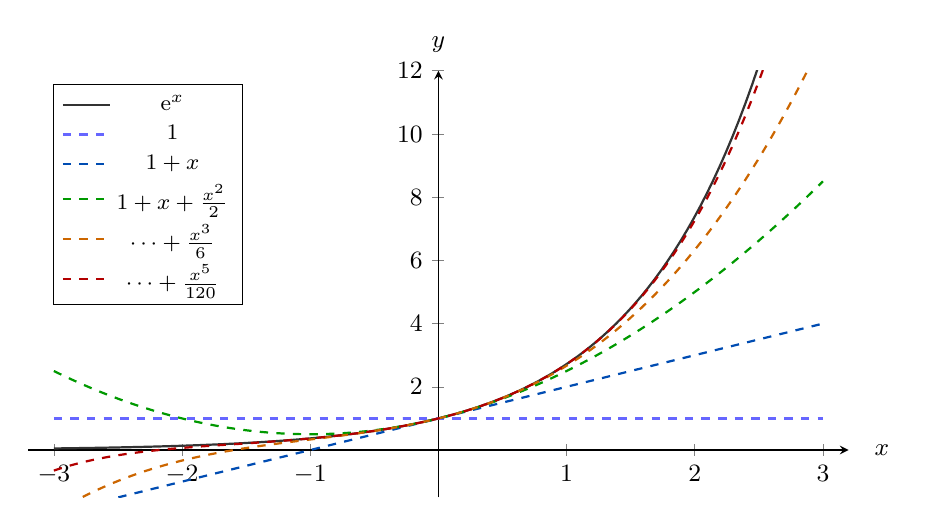
\begin{tikzpicture}
\begin{axis}[width=12cm, height=7cm, xmin=-3.2, xmax=3.2, ymin=-1.5, ymax=12,
  xlabel={$x$}, ylabel={$y$}, legend pos=north west, legend style={font=\footnotesize},
  samples=120, domain=-3:3, no markers, every axis plot/.append style={thick}]
  \addplot[black!80] {exp(x)};
  \addplot[blue!60, dashed] {1};
  \addplot[blue!70!green, dashed] {1+x};
  \addplot[green!60!black, dashed] {1+x+x^2/2};
  \addplot[orange!80!black, dashed] {1+x+x^2/2+x^3/6};
  \addplot[red!70!black, dashed] {1+x+x^2/2+x^3/6+x^4/24+x^5/120};
  \legend{$\e^x$, $1$, $1+x$, $1+x+\frac{x^2}{2}$, $\cdots+\frac{x^3}{6}$, $\cdots+\frac{x^5}{120}$}
\end{axis}
\end{tikzpicture}
\caption{$\e^x$ 的級數部分和。每多加一項，曲線在更大的範圍內貼近 $\e^x$。
在 $x=1$ 處，前 $13$ 項的和已經是 $2.7182818283$，和 $\e$ 的前十位小數相同。}
\label{fig:expseries}
\end{figure}

\begin{prereq}{從級數推出 $\e^{a+b}=\e^a\e^b$}
論文多次使用「指數律」$\e^{a+b}=\e^{a}\e^{b}$（第一節算 $B_r$ 時，以及第三節的命題 3.6）。
它可以直接從級數和\textbf{二項式定理}推出：
\begin{align*}
  \e^{a+b}=\sum_{n\ge0}\frac{(a+b)^n}{n!}
  &=\sum_{n\ge0}\sum_{k=0}^{n}\frac{1}{n!}\binom{n}{k}a^kb^{n-k}
  =\sum_{n\ge0}\sum_{k=0}^{n}\frac{a^k}{k!}\cdot\frac{b^{n-k}}{(n-k)!}\\
  &=\Big(\sum_{k\ge0}\frac{a^k}{k!}\Big)\Big(\sum_{l\ge0}\frac{b^l}{l!}\Big)=\e^a\e^b\,.
\end{align*}

中間用了 $\frac{1}{n!}\binom nk=\frac{1}{k!\,(n-k)!}$，最後一步是把「所有 $(k,l)$ 的乘積」
按 $k+l=n$ 分組。這種「重新分組」在第 \ref{sec:fps} 節會再出現，它正是兩個冪級數相乘的規則。
\end{prereq}

另一個會用到的性質：$\e^x$ 的導數還是 $\e^x$。逐項微分
$\big(\tfrac{x^n}{n!}\big)'=\tfrac{x^{n-1}}{(n-1)!}$，所以整個級數微分後只是「每一項往前移一格」，
形狀不變。於是 $(\e^{-x})'=-\e^{-x}$，這在第 \ref{sec:calc} 節的分部積分裡會用到。

\subsection{階乘打敗指數：$c^r/r!\to0$}\label{sec:factorial}

三個證明最後都靠同一個事實收尾：\emph{階乘的成長速度終究會超過任何固定底數的指數。}

\begin{prereq}{$c^r/r!\to0$}
固定任何一個實數 $c\ge1$。當 $r\to\infty$ 時，$\dfrac{c^r}{r!}\to0$。

\textbf{理由。}取一個整數 $R>2c$。當 $r\ge R$ 時，
\[
  \frac{c^{r}}{r!}=\frac{c^{R}}{R!}\cdot\frac{c}{R+1}\cdot\frac{c}{R+2}\cdots\frac{c}{r}
  \le\frac{c^{R}}{R!}\cdot\Big(\frac12\Big)^{r-R}\,,
\]
因為每個額外的因子 $\frac{c}{R+j}$ 都小於 $\frac12$。右邊是一個固定常數乘上 $(\tfrac12)^{r-R}$，
當然趨近於 $0$。同理，對任何固定的 $A\ge1$，當 $k$ 夠大時 $k!>A^k$；
論文第二節需要的形式是：存在 $k_0$，使得 $k\ge k_0$ 時 $k!>c\,A^{2tk}C^{k}=c\,(A^{2t}C)^k$。
\end{prereq}

\begin{figure}[htbp]
\centering
\begin{tikzpicture}
\begin{axis}[width=12cm, height=6.8cm, xmin=0, xmax=41, ymin=0, ymax=50,
  xlabel={$r$}, ylabel={$\log_{10}$（位數）}, legend pos=north west,
  legend style={font=\footnotesize}, no markers, every axis plot/.append style={thick}]
  \addplot[blue!70!black, domain=0:40, samples=2] {x};
  \addplot[red!70!black, mark=*, mark size=1pt] coordinates {
    (0,0.000) (1,0.000) (2,0.301) (3,0.778) (4,1.380) (5,2.079) (6,2.857) (7,3.702)
    (8,4.606) (9,5.560) (10,6.560) (11,7.601) (12,8.680) (13,9.794) (14,10.940)
    (15,12.116) (16,13.321) (17,14.551) (18,15.806) (19,17.085) (20,18.386)
    (21,19.708) (22,21.051) (23,22.412) (24,23.793) (25,25.191) (26,26.606)
    (27,28.037) (28,29.484) (29,30.947) (30,32.424) (31,33.915) (32,35.420)
    (33,36.939) (34,38.470) (35,40.014) (36,41.571) (37,43.139) (38,44.719)
    (39,46.310) (40,47.912)};
  \legend{$10^{r}$, $r!$}
  \draw[dashed, gray] (axis cs:25,0) -- (axis cs:25,25.2);
  \node[font=\footnotesize, anchor=west] at (axis cs:25.5,8) {$r=25$ 之後 $r!$ 反超};
\end{axis}
\end{tikzpicture}
\caption{以 $c=10$ 為例，比較 $10^{r}$ 與 $r!$ 的位數。$10^r$ 每多一步只多一位，
$r!$ 每多一步多 $\log_{10}r$ 位，越走越快。}
\label{fig:factorial}
\end{figure}

\subsection{暖身：核心招數，用它證明 $\e$ 是無理數}\label{sec:irrational}

三個證明的靈魂都是下面這個招數。我們先用它做一件高中生做得到的事。

\begin{keyidea}[核心招數：非零整數的絕對值至少是 $1$]
如果你能證明某個數 $N$ 同時滿足
\begin{enumerate}
  \item $N$ 是整數，而且 $N\neq0$；
  \item $|N|<1$，
\end{enumerate}
那就矛盾了。希爾伯特證明裡的 $N$ 是 $B_r/r!$（或等價地 $-A_r/r!$），
第二節的 $N$ 是 $v_n(k)/k!$。
\end{keyidea}

\begin{thm}[Fourier, 1815]
$\e$ 是無理數。
\end{thm}
\begin{pf}
假設 $\e=\dfrac{p}{q}$，$p,q\in\N$。把 $\e=\sum_{n\ge0}\frac1{n!}$ 乘上 $q!$：
\[
  q!\,\e=\underbrace{q!\Big(1+1+\frac1{2!}+\cdots+\frac1{q!}\Big)}_{\text{整數，記作 }M}
        +\underbrace{q!\Big(\frac{1}{(q+1)!}+\frac{1}{(q+2)!}+\cdots\Big)}_{\text{記作 }T}\,.
\]
左邊 $q!\,\e=(q-1)!\,p$ 是整數，$M$ 是整數，所以 $T=q!\,\e-M$ 也是整數。但是
\[
  0<T=\frac{1}{q+1}+\frac{1}{(q+1)(q+2)}+\cdots<\frac1{q+1}+\frac1{(q+1)^2}+\cdots=\frac1q\le1\,.
\]
$T$ 是嚴格介於 $0$ 與 $1$ 之間的整數，矛盾。
\end{pf}

請注意這個證明的骨架：「乘上一個大階乘，把級數拆成\emph{整數部分}與\emph{尾巴}，
尾巴非零但比 $1$ 小」。希爾伯特的證明是它的加強版：把「乘上 $q!$」換成「乘上一個
精心設計的積分」，讓拆出來的整數部分是 $r!$ 的倍數，而尾巴只有 $c^r$ 那麼大。
第二節的證明也是同一骨架，只是把「尾巴很小」這件事藏在 $v_n=O(A^n)$ 裡。

\section{積分、廣義積分，與歐拉的恆等式}\label{sec:calc}

希爾伯特的證明（論文第一節）和 Klazar 的證明（第三節）都圍繞著積分
$\int_0^{+\infty}p(x)\e^{-x}\dd x$。這一節把需要的積分知識補齊。
學過數學甲的同學知道「多項式的積分」，但「積分到無窮遠」與「分部積分」不在課綱內。

\subsection{積分、微積分基本定理、分部積分}

\begin{prereq}{定積分與微積分基本定理}
對於區間 $[a,b]$ 上的連續函數 $f$，$\int_a^b f(x)\dd x$ 是曲線 $y=f(x)$ 與 $x$ 軸之間
在 $a\le x\le b$ 的「有號面積」（$x$ 軸上方算正、下方算負）。
\textbf{微積分基本定理}說：如果 $F'(x)=f(x)$（$F$ 叫做 $f$ 的\emph{原函數}或\emph{反導函數}），那麼
\[
  \int_a^b f(x)\dd x=F(b)-F(a)\,.
\]
例如 $\int_0^2 x^2\dd x=\frac{2^3}{3}-0=\frac83$，因為 $\big(\frac{x^3}{3}\big)'=x^2$。
積分有\textbf{線性}：$\int(\alpha f+\beta g)=\alpha\int f+\beta\int g$；
也有\textbf{可加性}：$\int_a^c=\int_a^b+\int_b^c$（把面積切成兩塊）。
\end{prereq}

\begin{prereq}{分部積分（integration by parts）}
乘積的微分法則 $(uv)'=u'v+uv'$ 兩邊積分，得
\[
  \int_a^b u(x)v'(x)\dd x=\Big[u(x)v(x)\Big]_a^b-\int_a^b u'(x)v(x)\dd x\,,
  \qquad\text{其中 }\Big[uv\Big]_a^b:=u(b)v(b)-u(a)v(a)\,.
\]
它的用途是「把微分從一個因子搬到另一個因子上」。下面算 $\int x^n\e^{-x}$ 時，
就是把 $x^n$ 的次數一次降一。
\end{prereq}

\subsection{積分到無窮遠：廣義積分}

\begin{prereq}{廣義積分（improper integral）}
\[
  \int_0^{+\infty}f(x)\dd x:=\lim_{b\to+\infty}\int_0^{b}f(x)\dd x\,,
\]
只要這個極限存在（是一個有限的實數）。直覺上，它是一塊「向右無限延伸、但總面積有限」的區域。
同樣有線性與可加性：$\int_0^{+\infty}=\int_0^{j}+\int_j^{+\infty}$。
\end{prereq}

為什麼 $\int_0^{+\infty}x^n\e^{-x}\dd x$ 會是有限的？因為 $\e^{-x}$ 衰減得比任何多項式成長得快：
由級數 $\e^{x}\ge\dfrac{x^{n+2}}{(n+2)!}$（取級數中的一項，$x>0$），得
\[
  0<x^{n}\e^{-x}\le\frac{(n+2)!}{x^{2}}\qquad(x>0)\,,
\]
而 $\int_1^{b}\frac{1}{x^2}\dd x=1-\frac1b<1$ 有界，所以總面積有限。
順帶得到 $\lim_{x\to+\infty}x^n\e^{-x}=0$，等一下會用到。

\subsection{歐拉的恆等式：$\int_0^{+\infty}x^n\e^{-x}\dd x=n!$}

\begin{thm}[歐拉的恆等式]\label{thm:euler}
對所有 $n\in\N_0$，
\[
  I_n:=\int_0^{+\infty}x^n\e^{-x}\dd x=n!\,.
\]
\end{thm}
\begin{pf}
對 $n$ 做\textbf{數學歸納法}。$n=0$：$(-\e^{-x})'=\e^{-x}$，所以
$I_0=\lim_{b\to\infty}\big[-\e^{-x}\big]_0^{b}=\lim_{b\to\infty}(1-\e^{-b})=1=0!$。
設 $n\ge1$。分部積分，取 $u=x^n$、$v=-\e^{-x}$（則 $v'=\e^{-x}$）：
\[
  \int_0^{b}x^n\e^{-x}\dd x=\Big[-x^n\e^{-x}\Big]_0^{b}+n\int_0^{b}x^{n-1}\e^{-x}\dd x
  =-b^n\e^{-b}+n\int_0^{b}x^{n-1}\e^{-x}\dd x\,.
\]
令 $b\to\infty$，第一項趨近 $0$，得 $I_n=n\,I_{n-1}=n\cdot(n-1)!=n!$。
\end{pf}

由線性，馬上得到論文裡的「推廣形式」：對任何整數係數多項式 $\sum_{j=0}^m b_jx^j$，
\begin{equation}\label{eq:euler-poly}
  \int_0^{+\infty}\Big(\sum_{j=0}^m b_jx^j\Big)\e^{-x}\dd x=\sum_{j=0}^m b_j\cdot j!\,.
\end{equation}
這個式子是希爾伯特證明的引擎：\emph{積分把 $x^j$ 變成 $j!$}。
如果多項式從 $x^{r}$ 項才開始（前面係數全為 $0$），右邊每一項都是 $r!$ 的倍數。

\begin{figure}[htbp]
\centering
\begin{tikzpicture}
\begin{axis}[width=12.5cm, height=7cm, xmin=0, xmax=12.5, ymin=0, ymax=1.5,
  xlabel={$x$}, ylabel={$y$}, legend pos=north east, legend style={font=\footnotesize},
  samples=200, domain=0:12.5, no markers, every axis plot/.append style={thick}]
  \addplot[name path=f2, green!60!black] {x^2*exp(-x)};
  \path[name path=axis] (axis cs:0,0) -- (axis cs:12.5,0);
  \addplot[green!60!black, opacity=0.18] fill between[of=f2 and axis, soft clip={domain=0:12.5}];
  \addplot[blue!70!black] {exp(-x)};
  \addplot[orange!80!black] {x*exp(-x)};
  \addplot[red!70!black] {x^3*exp(-x)};
  \legend{$x^2\e^{-x}$（面積 $2!=2$）, , $\e^{-x}$（面積 $0!=1$）, $x\e^{-x}$（面積 $1!=1$）, $x^3\e^{-x}$（面積 $3!=6$）}
\end{axis}
\end{tikzpicture}
\caption{歐拉的恆等式：曲線 $x^n\e^{-x}$ 下方從 $0$ 到 $+\infty$ 的面積恰好是 $n!$。
$n$ 越大，山峰越往右、越高，但尾巴終究被 $\e^{-x}$ 壓下去。}
\label{fig:euler}
\end{figure}

\subsection{平移換元：$\int_j^{+\infty}f(x)\dd x=\int_0^{+\infty}f(y+j)\dd y$}

希爾伯特證明的第三個等式用了「變數變換 $y=x-j$」。它的幾何意義很直觀：
把函數圖形整個往左平移 $j$ 單位，面積不變。

\begin{prereq}{平移換元}
對任何連續函數 $f$ 與實數 $j$，
\[
  \int_j^{b}f(x)\dd x=\int_0^{b-j}f(y+j)\dd y\,,\qquad
  \int_j^{+\infty}f(x)\dd x=\int_0^{+\infty}f(y+j)\dd y\,.
\]
理由：若 $F'=f$，則 $G(y):=F(y+j)$ 滿足 $G'(y)=f(y+j)$（連鎖律），所以兩邊都等於 $F(b)-F(j)$。
\end{prereq}

\begin{figure}[htbp]
\centering
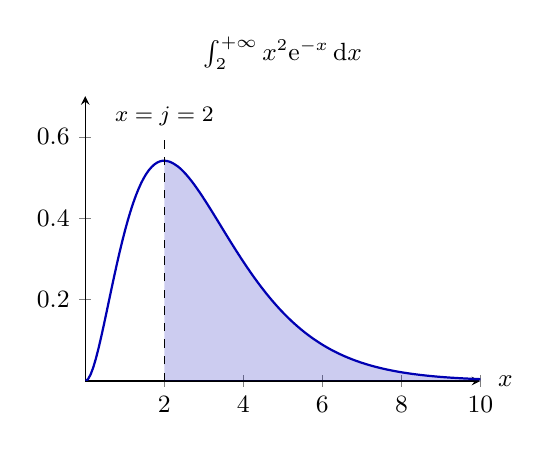
\begin{tikzpicture}
\begin{axis}[width=6.6cm, height=5.2cm, xmin=0, xmax=10, ymin=0, ymax=0.7,
  xlabel={$x$}, title={$\int_2^{+\infty}x^2\e^{-x}\dd x$}, title style={font=\small},
  samples=150, domain=0:10, no markers, every axis plot/.append style={thick}]
  \addplot[name path=f, blue!70!black] {x^2*exp(-x)};
  \path[name path=ax] (axis cs:0,0) -- (axis cs:10,0);
  \addplot[blue!70!black, opacity=0.2] fill between[of=f and ax, soft clip={domain=2:10}];
  \draw[dashed] (axis cs:2,0) -- (axis cs:2,0.6);
  \node[font=\footnotesize] at (axis cs:2,0.65) {$x=j=2$};
\end{axis}
\end{tikzpicture}
\hfill
\begin{tikzpicture}
\begin{axis}[width=6.6cm, height=5.2cm, xmin=0, xmax=10, ymin=0, ymax=0.7,
  xlabel={$y$}, title={$\int_0^{+\infty}(y+2)^2\e^{-(y+2)}\dd y$}, title style={font=\small},
  samples=150, domain=0:10, no markers, every axis plot/.append style={thick}]
  \addplot[name path=g, orange!80!black] {(x+2)^2*exp(-(x+2))};
  \path[name path=ax] (axis cs:0,0) -- (axis cs:10,0);
  \addplot[orange!80!black, opacity=0.2] fill between[of=g and ax, soft clip={domain=0:10}];
  \draw[arr, gray] (axis cs:5,0.5) -- (axis cs:3,0.5);
  \node[font=\footnotesize, anchor=west] at (axis cs:5.1,0.5) {圖形左移 $2$};
\end{axis}
\end{tikzpicture}
\caption{平移換元。左右兩塊著色區域是同一塊面積，只是右圖把起點移到了 $0$。
在希爾伯特證明裡，$f(y+j)=p_r(y+j)\e^{-(y+j)}=\e^{-j}\,p_r(y+j)\e^{-y}$，
平移之後就能套用歐拉的恆等式。}
\label{fig:shift}
\end{figure}

\subsection{一個粗估：有限區間上的積分不會太大}

論文估計 $|A_r|\le c^{r}$ 時用的是最笨、也最可靠的估計：
\begin{prereq}{積分的絕對值估計}
若在 $[a,b]$ 上 $|f(x)|\le M$，則 $\Big|\int_a^b f(x)\dd x\Big|\le M\,(b-a)$。
（面積不會超過「最高高度 $\times$ 寬度」的長方形。）
\end{prereq}
在 $[0,n]$ 上，$\e^{-x}\le1$，而
\[
  |p_r(x)|=|x|^r\,|(x-1)\cdots(x-n)|^{r+1}\le n^{r}\,(n^{n})^{r+1}\,,
  \qquad\text{所以}\qquad
  \Big|\int_0^{j}p_r(x)\e^{-x}\dd x\Big|\le n\cdot n^{r}\,n^{n(r+1)}\,,
\]
是某個只和 $n$ 有關的常數的 $r$ 次方。這就是 $|A_r|\le c^r$ 的全部內容。


\section{形式冪級數、有理冪級數與極點}\label{sec:fps}

論文標題裡的「形式冪級數」（formal power series，FPS）是第二、三節的主角。
它的想法很簡單：\emph{一個寫不完的多項式}。

\subsection{什麼是形式冪級數}

\begin{prereq}{形式冪級數 $\R[[x]]$}
一個（實係數）\textbf{形式冪級數}是一個形如
\[
  f(x)=a_0+a_1x+a_2x^2+a_3x^3+\cdots=\sum_{n\ge0}a_nx^n\qquad(a_n\in\R)
\]
的「無窮多項式」。重點在「形式」兩個字：\textbf{$x$ 只是一個佔位符號，不是數}；
我們\emph{不}把數字代進 $x$，所以完全不必擔心「收不收斂」。
一個 FPS 的全部資訊就是它的係數序列 $(a_0,a_1,a_2,\ldots)$。
所有實係數 FPS 的集合記作 $\R[[x]]$；係數限制在 $\Z$、$\Q$、$\C$ 時分別記作
$\Z[[x]]$、$\Q[[x]]$、$\C[[x]]$。多項式 $\R[x]$ 是「從某一項起係數全為 $0$」的 FPS。

\textbf{記號} $\coef{n}f$ 表示 $f$ 的 $x^n$ 係數，即 $\coef{n}f=a_n$。
\end{prereq}

\begin{prereq}{FPS 的四則與微積分（全部只是「對係數做事」）}
令 $f=\sum a_nx^n$，$g=\sum b_nx^n$。
\begin{itemize}
  \item \textbf{加法}：$\coef{n}(f+g)=a_n+b_n$。
  \item \textbf{乘法}：像多項式一樣展開再合併同類項，
        \[
          \coef{n}(fg)=a_0b_n+a_1b_{n-1}+\cdots+a_nb_0=\sum_{k=0}^{n}a_kb_{n-k}\,.
        \]
        每個係數都是\emph{有限}的和，所以永遠算得出來（見圖 \ref{fig:cauchy}）。
  \item \textbf{導數}：逐項微分，$f'=\sum_{n\ge0}(n+1)a_{n+1}x^n$。
        乘積法則 $(fg)'=f'g+fg'$ 仍然成立。
  \item \textbf{原函數}：逐項積分，$\int f:=\sum_{n\ge0}\dfrac{a_n}{n+1}x^{n+1}$（常數項取 $0$）。
        於是 $\big(\int f\big)'=f$，而 $\int f'=f-a_0$。
  \item \textbf{代入 $ax$}：$f(ax):=\sum a^na_nx^n$。例如 $f(-x)=a_0-a_1x+a_2x^2-\cdots$。
\end{itemize}
\end{prereq}

\begin{figure}[htbp]
\centering
\begin{tikzpicture}[font=\small]
  \matrix (m) [matrix of math nodes, nodes={minimum width=1.5cm, minimum height=0.8cm, anchor=center},
               column sep=1pt, row sep=1pt, nodes in empty cells] {
    & b_0 & b_1 & b_2 & b_3 \\
    a_0 & a_0b_0 & a_0b_1 & a_0b_2 & a_0b_3 \\
    a_1 & a_1b_0 & a_1b_1 & a_1b_2 & a_1b_3 \\
    a_2 & a_2b_0 & a_2b_1 & a_2b_2 & a_2b_3 \\
    a_3 & a_3b_0 & a_3b_1 & a_3b_2 & a_3b_3 \\
  };
  \begin{scope}[on background layer]
    \fill[blue!15] (m-2-2.north west) rectangle (m-2-2.south east);
    \fill[green!15] (m-2-3.north west) rectangle (m-2-3.south east);
    \fill[green!15] (m-3-2.north west) rectangle (m-3-2.south east);
    \fill[orange!18] (m-2-4.north west) rectangle (m-2-4.south east);
    \fill[orange!18] (m-3-3.north west) rectangle (m-3-3.south east);
    \fill[orange!18] (m-4-2.north west) rectangle (m-4-2.south east);
    \fill[red!15] (m-2-5.north west) rectangle (m-2-5.south east);
    \fill[red!15] (m-3-4.north west) rectangle (m-3-4.south east);
    \fill[red!15] (m-4-3.north west) rectangle (m-4-3.south east);
    \fill[red!15] (m-5-2.north west) rectangle (m-5-2.south east);
  \end{scope}
  \node[anchor=west, text=blue!60!black] at ([xshift=4mm]m-2-5.east) {};
  \node[right=0.9cm of m-3-5, align=left, text width=4.6cm] {
    同一條「反對角線」上 $k+l$ 相同，\\
    加起來就是 $\coef{n}(fg)$：\\[2pt]
    \textcolor{blue!60!black}{$n=0$}：$a_0b_0$\\
    \textcolor{green!50!black}{$n=1$}：$a_0b_1+a_1b_0$\\
    \textcolor{orange!80!black}{$n=2$}：$a_0b_2+a_1b_1+a_2b_0$\\
    \textcolor{red!70!black}{$n=3$}：$a_0b_3+a_1b_2+a_2b_1+a_3b_0$};
\end{tikzpicture}
\caption{兩個冪級數相乘。乘積的第 $n$ 個係數只用到 $a_0,\ldots,a_n$ 與 $b_0,\ldots,b_n$，
是有限和，不需要任何極限。第 \ref{sec:numbers} 節證明 $\e^{a+b}=\e^a\e^b$ 時的「重新分組」
正是這張圖。}
\label{fig:cauchy}
\end{figure}

\begin{exmp}[幾何級數與形式指數]
\begin{enumerate}
  \item $(1-x)(1+x+x^2+x^3+\cdots)=1$：按乘法規則，$n\ge1$ 的係數是 $1\cdot1+(-1)\cdot1=0$。
        所以在 $\R[[x]]$ 裡我們\emph{定義} $\dfrac{1}{1-x}:=1+x+x^2+\cdots$。
        這句話不牽涉任何收斂，純粹是代數；高中「無窮等比級數 $|x|<1$」的條件在這裡不需要。
  \item 論文定義 3.2 的\textbf{形式指數} $\Exp(x):=\sum_{n\ge0}\dfrac{x^n}{n!}\in\Q[[x]]$。
        逐項微分得 $\Exp'=\Exp$，逐項積分得 $\int\Exp=\Exp-1$。
        注意：$\Exp$ 是一串係數 $(1,1,\tfrac12,\tfrac16,\ldots)$，而 $\e^x$ 是函數；
        兩者在第 \ref{sec:klazar} 節才會被「半形式」運算連結起來。
\end{enumerate}
\end{exmp}

\begin{prereq}{收斂的 FPS：$\R\{x\}$}
有些 FPS 可以「代數字進去」：如果對\emph{每一個}實數 $b$，數列
$\sum_{n=0}^{N}a_nb^n$ 都在 $N\to\infty$ 時收斂，就說 $f$ 是\textbf{收斂的}（收斂半徑無窮大），
並把極限記作 $f(b)$。這種 FPS 的集合記作 $\R\{x\}$。$\Exp$ 與所有多項式都屬於 $\R\{x\}$，
而 $\frac1{1-x}=\sum x^n$ \emph{不}屬於（代 $b=2$ 就發散）。
論文第三節只在 $\R\{x\}$ 裡工作，因為它需要「代值」這個動作。
\end{prereq}

\subsection{有理冪級數、部分分式與極點}\label{sec:rational}

\begin{prereq}{有理 FPS}
$f\in\C[[x]]$ 叫做\textbf{有理的}，如果存在多項式 $p,q\in\C[x]$，$q(0)=1$，使得 $q(x)f(x)=p(x)$。
直覺：$f=\dfrac{p}{q}$ 是一個「分式」展開成的冪級數。
有理 FPS 的和、積、導數仍是有理的（通分、乘開、商的微分法則）。
\end{prereq}

\begin{exmp}\label{ex:pole}
$\dfrac{1}{1-2x}=\sum_{n\ge0}2^nx^n$（驗證：$(1-2x)\sum2^nx^n$ 的 $n\ge1$ 係數是 $2^n-2\cdot2^{n-1}=0$）。
把它看成函數時，在 $x=\tfrac12$ 分母為 $0$，圖形有垂直漸近線（圖 \ref{fig:pole}）；
這個點叫做\textbf{極點}（pole）。係數 $2^n$ 的成長速度正好反映極點的位置：
極點在 $1/\alpha$ 時，係數像 $\alpha^n$ 一樣成長。
\end{exmp}

\begin{figure}[htbp]
\centering
\begin{tikzpicture}
\begin{axis}[width=12cm, height=6.5cm, xmin=-1.6, xmax=1.6, ymin=-8, ymax=8,
  xlabel={$x$}, ylabel={$y$}, samples=300, no markers, restrict y to domain=-8:8,
  every axis plot/.append style={thick}]
  \addplot[blue!10, fill=blue!10, draw=none, domain=-0.5:0.5] {8} \closedcycle;
  \addplot[blue!10, fill=blue!10, draw=none, domain=-0.5:0.5] {-8} \closedcycle;
  \addplot[blue!70!black, domain=-1.6:0.49] {1/(1-2*x)};
  \addplot[blue!70!black, domain=0.51:1.6] {1/(1-2*x)};
  \draw[dashed, red!70!black, thick] (axis cs:0.5,-8) -- (axis cs:0.5,8);
  \node[font=\footnotesize, red!70!black, anchor=west] at (axis cs:0.55,6.5) {極點 $x=\frac12$};
  \node[font=\footnotesize, blue!60!black] at (axis cs:-0.05,-6.3) {級數 $\sum 2^nx^n$ 在此收斂};
  \draw[orange!80!black, thick, dashed, domain=-0.5:0.5, samples=50] plot (\x, {1+2*\x+4*\x*\x+8*\x*\x*\x});
\end{axis}
\end{tikzpicture}
\caption{$y=\dfrac{1}{1-2x}$ 與它的極點。橘色虛線是前四項 $1+2x+4x^2+8x^3$，
只在 $|x|<\frac12$（藍色帶）貼近曲線。在 FPS 的世界裡我們不代值，所以只需要記住：
「分母 $1-\alpha x$」$\leftrightarrow$「極點 $1/\alpha$」$\leftrightarrow$「係數成長 $\alpha^n$」。}
\label{fig:pole}
\end{figure}

\begin{prereq}{部分分式與極點的階}
高中學過把 $\dfrac{1}{(1-x)(1-2x)}$ 拆成 $\dfrac{-1}{1-x}+\dfrac{2}{1-2x}$。一般地，
若 $q(x)=\prod_{j=1}^{t}(1-\alpha_jx)^{m_j}$（$\alpha_j$ 互不相同、皆非零），則每個有理 FPS
$p/q$ 都可唯一寫成
\[
  f(x)=r(x)+\sum_{j=1}^{t}\sum_{i=1}^{m_j}\frac{\beta_{j,i}}{(1-\alpha_jx)^{i}}\,,
  \qquad r\in\C[x],\ \beta_{j,m_j}\neq0\,.
\]
我們說 $1/\alpha_j$ 是 $f$ 的\textbf{極點}，\textbf{階}（order）是 $m_j$，
也就是分母裡 $(1-\alpha_jx)$ 出現的最高次數。每個部分分式本身是 FPS：
\[
  \frac{1}{(1-\alpha x)^{i}}=\sum_{n\ge0}\binom{n+i-1}{i-1}\alpha^nx^n\,,
\]
例如 $\frac{1}{(1-\alpha x)^2}=\sum(n+1)\alpha^nx^n$。
（論文寫成 $\binom{-i}{n}(-\alpha)^n$ 的形式，兩者相同：
$\binom{-i}{n}:=\frac{(-i)(-i-1)\cdots(-i-n+1)}{n!}=(-1)^n\binom{n+i-1}{n}$。）
\end{prereq}

\begin{keyidea}[極點的階在運算下如何變化（論文命題 2.1 的全部內容）]
設 $A(x)$ 是有理 FPS，$1/\alpha$ 是它的 $m$ 階極點。
\begin{itemize}
  \item \textbf{微分讓階數加一}：$\Big(\dfrac{1}{(1-\alpha x)^m}\Big)'=\dfrac{m\alpha}{(1-\alpha x)^{m+1}}$。
        所以 $A'$ 在 $1/\alpha$ 有 $m+1$ 階極點。
  \item \textbf{乘上多項式不會製造新極點}，只可能降低階數或把極點消掉
        （若多項式含因子 $(1-\alpha x)$）。例如 $(1-\alpha x)\cdot\dfrac{1}{(1-\alpha x)^m}=\dfrac{1}{(1-\alpha x)^{m-1}}$。
  \item \textbf{相加時}，若兩個級數在同一點的階數不同，和的階數是較大的那個（高階項不可能被低階項消掉）。
\end{itemize}
把三點合起來：$p(x)A(x)+c\,x^{m}A'(x)$（$c\neq0$）的極點就是 $c\,x^mA'(x)$ 的極點，每個階數都至少 $2$；
除非 $A$ 根本是多項式。這就是論文的命題 2.1。
\end{keyidea}

\subsection{有理 $\Leftrightarrow$ 線性遞迴}

高中學過費氏數列 $F_0=0$、$F_1=1$、$F_n=F_{n-1}+F_{n-2}$。它的\textbf{生成函數}
$F(x)=\sum F_nx^n$ 滿足
\[
  (1-x-x^2)F(x)=x\,,
\]
因為左邊 $x^n$（$n\ge2$）的係數是 $F_n-F_{n-1}-F_{n-2}=0$。所以 $F(x)=\dfrac{x}{1-x-x^2}$ 是有理的。
反過來也對：
\begin{prereq}{有理 FPS 的係數滿足線性遞迴}
若 $q(x)=1-a_1x-\cdots-a_tx^t$ 且 $q(x)f(x)$ 是一個次數 $<d$ 的多項式，則 $f$ 的係數 $v_n$ 滿足
\[
  v_n=a_1v_{n-1}+a_2v_{n-2}+\cdots+a_tv_{n-t}\qquad(n\ge d)\,.
\]
理由：$\coef{n}\big(q(x)f(x)\big)=v_n-a_1v_{n-1}-\cdots-a_tv_{n-t}$，而它在 $n\ge d$ 時為 $0$。
\end{prereq}
論文定理 2.2 的結論「$q(x)^kV(x)\in\Z[x]$」，翻成白話就是：
\emph{$v_n$ 從某一項起滿足一個固定的線性遞迴}，係數來自 $q(x)^k$。
而要證明 FPS 有理，只要證明「乘上 $q^k$ 之後，從某一項起係數全為 $0$」。
這正是第 \ref{sec:bbr} 節的戰略。

\begin{prereq}{大 $O$ 記號}
「$v_n=O(A^n)$」的意思是：存在常數 $c>0$，使得對所有 $n$ 都有 $|v_n|\le c\,A^n$。
它只說「成長不超過指數 $A^n$ 的某個倍數」，不管那個倍數多大。
\end{prereq}

\section{可數與不可數：論文真正關心的事}\label{sec:countable}

論文第一節後半的討論，對高中生來說可能是最陌生的：作者說希爾伯特的證明
「實質上使用了不可數集合」，並想把它們消掉。要懂這句話，先得知道「可數」是什麼。

\subsection{可數集合}

\begin{prereq}{可數（countable）}
一個集合是\textbf{可數的}，如果它的元素可以\emph{排成一列}
$x_1,x_2,x_3,\ldots$（每個元素都在某個位置出現，可以有限也可以無限）。
換句話說，它的元素能和正整數 $1,2,3,\ldots$ 一一對應（或者更少）。
\end{prereq}

\begin{exmp}
\begin{itemize}
  \item $\N$ 當然可數。$\Z$ 也可數：排成 $0,1,-1,2,-2,3,-3,\ldots$。
  \item $\Q$ 可數，雖然有理數在數線上「密密麻麻」。圖 \ref{fig:zigzag} 給出排法。
  \item 可數集合的「有限多個」或「可數多個」聯集仍可數；可數集合的子集仍可數。
\end{itemize}
\end{exmp}

\begin{figure}[htbp]
\centering
\begin{tikzpicture}[font=\small, scale=1.0]
  \foreach \p in {1,...,5} {
    \foreach \q in {1,...,5} {
      \node (n\p\q) at (1.5*\q, -1.1*\p) {$\frac{\p}{\q}$};
    }
  }
  \draw[arr, red!70!black] (n11) -- (n12);
  \draw[arr, red!70!black] (n12) -- (n21);
  \draw[arr, red!70!black] (n21) -- (n31);
  \draw[arr, red!70!black] (n31) -- (n22);
  \draw[arr, red!70!black] (n22) -- (n13);
  \draw[arr, red!70!black] (n13) -- (n14);
  \draw[arr, red!70!black] (n14) -- (n23);
  \draw[arr, red!70!black] (n23) -- (n32);
  \draw[arr, red!70!black] (n32) -- (n41);
  \draw[arr, red!70!black] (n41) -- (n51);
  \draw[arr, red!70!black] (n51) -- (n42);
  \draw[arr, red!70!black] (n42) -- (n33);
  \draw[arr, red!70!black] (n33) -- (n24);
  \draw[arr, red!70!black] (n24) -- (n15);
  \node[anchor=west, align=left, text width=5.2cm] at (8.6,-3.3) {
    沿著箭頭走，每一個正有理數都會被走到（重複的像 $\frac22=\frac11$ 跳過即可）。\\[3pt]
    走到的順序：$1,\frac12,2,3,\frac22,\frac13,\frac14,\frac23,\frac32,4,\ldots$\\[3pt]
    所以正有理數可以排成一列：$\Q$ 是可數的。};
\end{tikzpicture}
\caption{把正有理數排成一列（Cantor 的「之」字形走法）。}
\label{fig:zigzag}
\end{figure}

\subsection{實數不可數：Cantor 的對角線}

\begin{thm}[Cantor, 1874/1891]
區間 $[0,1)$ 裡的實數\emph{不可數}。
\end{thm}
\begin{pf}[證明（對角線論證）]
假設 $[0,1)$ 的所有實數可以排成一列 $x_1,x_2,x_3,\ldots$，把每個數寫成無窮小數
（規定不用 $9$ 循環的寫法，使寫法唯一）：
\[
  x_1=0.\,\mathbf{d_{11}}\,d_{12}\,d_{13}\ldots,\quad
  x_2=0.\,d_{21}\,\mathbf{d_{22}}\,d_{23}\ldots,\quad
  x_3=0.\,d_{31}\,d_{32}\,\mathbf{d_{33}}\ldots,\quad\ldots
\]
造一個新數 $y=0.\,c_1c_2c_3\ldots$，規定 $c_n=5$ 若 $d_{nn}\neq5$、$c_n=6$ 若 $d_{nn}=5$。
則 $y$ 的第 $n$ 位和 $x_n$ 的第 $n$ 位不同，所以 $y\neq x_n$ 對每個 $n$ 都成立，
$y$ 不在列表裡。矛盾。
\end{pf}

\begin{figure}[htbp]
\centering
\begin{tikzpicture}[font=\small]
  \matrix (m) [matrix of nodes, nodes={minimum width=0.75cm, minimum height=0.7cm, anchor=center},
               column sep=1pt, row sep=1pt] {
    $x_1=0.$ & 3 & 1 & 4 & 1 & 5 & $\cdots$ \\
    $x_2=0.$ & 7 & 0 & 7 & 1 & 0 & $\cdots$ \\
    $x_3=0.$ & 1 & 4 & 1 & 4 & 2 & $\cdots$ \\
    $x_4=0.$ & 5 & 0 & 0 & 0 & 0 & $\cdots$ \\
    $x_5=0.$ & 2 & 7 & 1 & 8 & 2 & $\cdots$ \\
    $\vdots$ & & & & & & \\
    $y\;=0.$ & 5 & 5 & 5 & 5 & 5 & $\cdots$ \\
  };
  \begin{scope}[on background layer]
    \foreach \i in {1,...,5} {
      \pgfmathtruncatemacro{\j}{\i+1}
      \fill[red!18] (m-\i-\j.north west) rectangle (m-\i-\j.south east);
    }
    \fill[blue!12] (m-7-2.north west) rectangle (m-7-6.south east);
  \end{scope}
  \node[anchor=west, text width=5.4cm, align=left] at ([xshift=6mm]m-3-7.east)
    {紅色是對角線上的數字 $d_{nn}$。\\ 新數 $y$ 的第 $n$ 位故意和 $d_{nn}$ 不同（這裡 $d_{nn}\ne5$ 就填 $5$，
     $d_{nn}=5$ 就填 $6$），所以 $y$ 和列表裡的每一個數都至少差一位。};
\end{tikzpicture}
\caption{對角線論證。不論怎麼列，都會漏掉某個實數，所以實數排不成一列。}
\label{fig:diagonal}
\end{figure}

\subsection{「函數」是不可數集合，「係數序列」是可數的}

在集合論裡，一個函數 $F\colon[0,+\infty)\to\R$ 被\emph{定義為}所有點對
$\langle x,F(x)\rangle$ 組成的集合，也就是它的圖形。
定義域 $[0,+\infty)$ 不可數，所以這個集合不可數。
希爾伯特的證明用了函數 $F(x)=p(x)\e^{-x}$ 以及它的積分，
作者說這就是證明裡「實質上使用不可數集合」的地方。

那麼什麼是「可數的替代品」？論文借希爾伯特之口說（第一節末）：
\emph{這些函數很特別，它們都是冪級數 $F(x)=\sum a_nx^n$，
而係數序列 $(a_0,a_1,a_2,\ldots)$ 是可數的。要算 $F(b)$ 就算極限 $\lim_N\sum_{n\le N}a_nb^n$。
把 $F$ 換成 $(a_0,a_1,\ldots)$ 就行了。}

\begin{figure}[htbp]
\centering
\begin{tikzpicture}[font=\small]
  \begin{scope}
    \draw[arr] (-0.3,0) -- (5,0) node[below] {$x$};
    \draw[arr] (0,-0.3) -- (0,3) node[left] {$y$};
    \draw[thick, blue!70!black, domain=0:4.8, samples=80] plot (\x, {2.6*\x*\x*exp(-\x)});
    \foreach \x in {0.3,0.7,1.1,1.5,1.9,2.3,2.7,3.1,3.5,3.9,4.3} {
      \fill[blue!70!black] (\x, {2.6*\x*\x*exp(-\x)}) circle (1.2pt);
    }
    \node[text width=4.6cm, align=center] at (2.4,-1.0) {函數 $F$ $=$ 所有點對 $\langle x,F(x)\rangle$ 的集合\\ \textbf{不可數}};
  \end{scope}
  \draw[arr, very thick, gray] (5.6,1.3) -- (7.0,1.3) node[midway, above, font=\footnotesize] {換成};
  \begin{scope}[xshift=7.6cm]
    \foreach \i/\v in {0/a_0,1/a_1,2/a_2,3/a_3,4/a_4} {
      \node[draw, rounded corners=2pt, minimum width=0.9cm, minimum height=0.8cm, fill=orange!10]
        at (1.0*\i, 1.3) {$\v$};
    }
    \node at (5.3,1.3) {$\cdots$};
    \node[text width=5.2cm, align=center] at (2.6,-1.0) {係數序列 $(a_0,a_1,a_2,\ldots)$\\ \textbf{可數}（而且每個 $a_n$ 也可用可數物件表示）};
  \end{scope}
\end{tikzpicture}
\caption{同一個資訊的兩種包裝。左邊的圖形有不可數多個點；右邊是一列數字。
論文第三節要做的，就是證明希爾伯特證明裡的每一步都能只用右邊的包裝完成。}
\label{fig:function-vs-sequence}
\end{figure}

\subsection{「遺傳可數」與戴德金分割}

論文提出四點說明，其中第 3、4 點用了兩個名詞：

\begin{prereq}{遺傳可數（hereditarily countable）與戴德金分割（Dedekind cut）}
\begin{itemize}
  \item 一個集合是\textbf{遺傳可數}的，如果它本身可數，它的每個元素（若是集合）也可數，
        元素的元素也可數……一路到底。這是比「可數」更嚴格的要求：
        例如 $\{\R\}$ 只有一個元素，當然可數，但它的元素 $\R$ 不可數，所以不是遺傳可數。
  \item 為了讓「實數」本身是可數的物件，論文把每個實數 $b$ 表示成\textbf{戴德金分割}：
        所有小於 $b$ 的有理數所成的集合 $\{q\in\Q: q<b\}$。因為 $\Q$ 可數，這個集合可數；
        而它完全決定了 $b$（例如 $\sqrt2$ 對應 $\{q\in\Q: q<0\text{ 或 }q^2<2\}$）。
\end{itemize}
於是「一串實數 $(a_0,a_1,\ldots)$」是遺傳可數的：它是可數多個可數集合排成一列。
\end{prereq}

\begin{rem}
論文也坦白說，「實質使用」（substantial use）這個詞沒有精確定義，只能靠直覺判斷：
像「對所有 $|x|<1$ 的實數 $x$，$\sum x^n=\frac1{1-x}$」雖然提到 $\R$，
但這句話可以輕易改寫成不提 $\R$ 的形式，所以不算實質使用。
另外，數理邏輯早就知道（Weyl 1918 年起）整個實分析可以在「二階算術」裡進行，
本來就是可數的事業；但論文想要的是\emph{不需要懂數理邏輯}、技術上更簡單的做法。
這是一種數學家的品味，而不是對錯問題；高中生讀到這裡，只需知道「有人在意這件事」即可。
\end{rem}

\subsection{其他會用到的小工具}

\begin{prereq}{下降階乘與組合數}
記 $(n)_0=1$，$(n)_m=n(n-1)\cdots(n-m+1)$（$m$ 個連續遞減的因子）。則
\[
  (n)_m=m!\binom{n}{m}\qquad(n\ge m)\,,
\]
且 $n<m$ 時 $(n)_m=0$（因為乘到了 $0$）。
論文第二節反覆用「$(n)_k$ 是 $k!$ 的倍數」這件事。
\end{prereq}

\begin{prereq}{Vandermonde 恆等式}
\[
  \sum_{k=0}^{n}\binom{m}{k}\binom{l}{n-k}=\binom{m+l}{n}\,.
\]
理由（算兩次）：從 $m$ 個男生、$l$ 個女生中選出 $n$ 人；右邊直接選，左邊按「男生選了 $k$ 人」分類。
論文命題 3.5 用它證明「平移」和「乘法」可以交換。
\end{prereq}

\begin{prereq}{質數無窮多，與互質}
對任何整數 $m\ge1$，都有無窮多個質數 $p$ 與 $m$ 互質（事實上所有大於 $m$ 的質數都行）。
希爾伯特證明用它挑出無窮多個 $r$，使 $r+1$ 與 $a_0\cdot n!$ 互質。
\end{prereq}

\clearpage
\part{論文第一節：希爾伯特的證明，以及為什麼要「可數化」}
\section{希爾伯特的證明，一步一步}\label{sec:hilbert}

這一節對應論文第一節的前半（到 $\Box$ 為止）。有了第 \ref{sec:calc} 節的工具，
整個證明可以在兩頁內講完，但每一步的「為什麼這樣設計」值得慢慢看。

\begin{keyidea}[希爾伯特證明的藍圖]
假設 $P:=a_0+a_1\e+\cdots+a_n\e^n=0$（整數係數，$a_0\neq0$）。對每個 $r\in\N$，
造一個積分 $I_r=\int_0^{+\infty}p_r(x)\e^{-x}\dd x$，然後把 $0=P\cdot I_r$ 拆成兩塊：
\[
  0=P\,I_r=\underbrace{A_r}_{\text{「小量」：}|A_r|\le c^r}
         +\underbrace{B_r}_{\text{「整數」：}r!\text{ 的倍數，且對無窮多個 }r\text{ 非零}}\,.
\]
於是對無窮多個 $r$，$r!\le|B_r|=|A_r|\le c^{r}$，與 $c^r/r!\to0$ 矛盾。
這就是第 \ref{sec:irrational} 節的核心招數，$N=B_r/r!$。
\end{keyidea}

\begin{figure}[htbp]
\centering
\begin{tikzpicture}[node distance=0.55cm and 0.8cm, font=\small]
  \node[box, fill=red!6, text width=5.4cm] (h) {\textbf{反證假設}\\ $P=a_0+a_1\e+\cdots+a_n\e^n=0$，$a_0\ne0$};
  \node[box, fill=gray!8, text width=5.4cm, below=of h] (p) {\textbf{設計多項式}\\ $p_r(x)=x^{r}\big((x-1)\cdots(x-n)\big)^{r+1}$\\
     {\footnotesize 在 $0$ 有 $r$ 重根，在 $1,\ldots,n$ 有 $r{+}1$ 重根}};
  \node[box, fill=gray!8, text width=5.4cm, below=of p] (i) {\textbf{乘上積分}\\ $0=P\cdot\displaystyle\int_0^{+\infty}p_r(x)\e^{-x}\dd x$\\
     把第 $j$ 項的積分從 $j$ 切開：$\int_0^{j}+\int_j^{+\infty}$};
  \node[box, fill=blue!8, text width=4.3cm, below left=0.8cm and -1.6cm of i] (a) {\textbf{$A_r=\sum a_j\e^{j}\int_0^{j}$}\\ 有限區間，粗估即可\\ $|A_r|\le c^{r}$};
  \node[box, fill=orange!10, text width=4.6cm, below right=0.8cm and -1.6cm of i] (b) {\textbf{$B_r=\sum a_j\e^{j}\int_j^{+\infty}$}\\ 平移 $+$ 歐拉恆等式\\ $B_r=\pm a_0(n!)^{r+1}r!+m_r(r+1)!$};
  \node[box, fill=green!10, text width=5.6cm, anchor=north] (c) at ($(a.south)!0.5!(b.south)+(0,-0.7cm)$) {\textbf{矛盾}\\ 取 $r+1$ 為大質數 $\Rightarrow B_r\neq0$，於是\\ $r!\le|B_r|=|A_r|\le c^{r}$，但 $c^r/r!\to0$};

  \draw[arr] (h) -- (p); \draw[arr] (p) -- (i);
  \draw[arr] (i) -- (a); \draw[arr] (i) -- (b);
  \draw[arr] (a) -- (c); \draw[arr] (b) -- (c);
\end{tikzpicture}
\caption{希爾伯特證明的流程。}
\label{fig:hilbert-flow}
\end{figure}

\subsection{第 0 步：為什麼可以假設 $a_0\neq0$}

若 $a_0=0$，整個式子可以提出一個 $\e$ 來：$\e(a_1+a_2\e+\cdots)=0$，因為 $\e\neq0$，
括號裡仍是 $0$，而且次數少了一。重複直到常數項非零即可。

\subsection{第 1 步：多項式 $p_r(x)$ 的設計}

\[
  p_r(x)=x^{r}\big((x-1)(x-2)\cdots(x-n)\big)^{r+1}\,.
\]
它的設計目的全在「根的重數」（圖 \ref{fig:roots}）：
\begin{itemize}
  \item 在 $x=0$ 是 $r$ 重根：展開後最低次項是 $x^{r}$，係數是
        \[
          \big((-1)(-2)\cdots(-n)\big)^{r+1}=(-1)^{n(r+1)}(n!)^{r+1}\,,
        \]
        所以 $p_r(x)=\pm(n!)^{r+1}x^{r}+(\text{更高次項})$。
  \item 在 $x=j$（$j=1,\ldots,n$）是 $r+1$ 重根：把 $x$ 換成 $x+j$ 後，
        因子 $(x+j-j)^{r+1}=x^{r+1}$ 出現，所以 $p_r(x+j)=b\,x^{r+1}+c\,x^{r+2}+\cdots$，
        最低次是 $x^{r+1}$，係數都是整數。
\end{itemize}
配合歐拉恆等式「積分把 $x^{m}$ 變成 $m!$」，第一點會產生一個「恰好是 $r!$ 倍、但不是 $(r+1)!$ 倍」的項，
第二點產生的全是 $(r+1)!$ 的倍數。這個「$r!$ 與 $(r+1)!$ 的落差」就是整個證明的槓桿。

\begin{figure}[htbp]
\centering
\begin{tikzpicture}[font=\small]
  \draw[arr] (-0.8,0) -- (8.2,0) node[below] {$x$};
  \foreach \x/\l in {0/0,2/1,4/2,6/$n$} { \draw (\x,0.1) -- (\x,-0.1) node[below] {\l}; }
  \node at (5,-0.35) {$\cdots$};
  \fill[blue!70!black] (0,0) circle (3pt);
  \node[above, blue!70!black, align=center] at (0,0.25) {$r$ 重根\\ {\footnotesize $x^{r}$}};
  \foreach \x in {2,4,6} {
    \fill[orange!80!black] (\x,0) circle (3pt);
    \node[above, orange!80!black, align=center] at (\x,0.25) {$r{+}1$ 重根\\ {\footnotesize $(x-j)^{r+1}$}};
  }
\end{tikzpicture}
\caption{$p_r(x)$ 的根。重根越多，多項式在該點附近「貼地」越久，這也是 $A_r$ 很小的直覺原因：
在 $[0,n]$ 上 $p_r$ 一直被壓在 $0$ 附近。}
\label{fig:roots}
\end{figure}

\subsection{第 2 步：把 $0=P\,I_r$ 拆成 $A_r+B_r$}

$I_r=\int_0^{+\infty}p_r(x)\e^{-x}\dd x$ 存在（第 \ref{sec:calc} 節）。於是
\[
  0=P\,I_r=\sum_{j=0}^{n}a_j\e^{j}\int_0^{+\infty}p_r(x)\e^{-x}\dd x
  =\underbrace{\sum_{j=0}^{n}a_j\e^{j}\int_0^{j}p_r(x)\e^{-x}\dd x}_{A_r}
  +\underbrace{\sum_{j=0}^{n}a_j\e^{j}\int_j^{+\infty}p_r(x)\e^{-x}\dd x}_{B_r}\,,
\]
第 $j$ 項的積分從 $x=j$ 切成兩段（可加性）。$j=0$ 那一項的 $\int_0^0=0$，全部歸到 $B_r$。

\begin{figure}[htbp]
\centering
\begin{tikzpicture}
\begin{axis}[width=13cm, height=6.8cm, xmin=0, xmax=14.5, ymin=0, ymax=6.8,
  xlabel={$x$}, ylabel={$y$}, samples=300, domain=0:14.5, no markers,
  every axis plot/.append style={thick}, legend pos=north east, legend style={font=\footnotesize}]
  \addplot[name path=f, black!80] {x*((x-1)*(x-2))^2*exp(-x)};
  \path[name path=ax] (axis cs:0,0) -- (axis cs:14.5,0);
  \addplot[blue!60, opacity=0.35] fill between[of=f and ax, soft clip={domain=0:1}];
  \addplot[orange!80, opacity=0.35] fill between[of=f and ax, soft clip={domain=1:14.5}];
  \draw[dashed, red!70!black] (axis cs:1,0) -- (axis cs:1,6.5);
  \node[font=\footnotesize, red!70!black, anchor=west] at (axis cs:1.1,6.2) {$x=j=1$：切開點};
  \node[font=\footnotesize, blue!60!black, anchor=west] at (axis cs:0.2,1.2) {$\int_0^{1}$（進 $A_r$，很小）};
  \node[font=\footnotesize, orange!80!black] at (axis cs:7.5,2.2) {$\int_1^{+\infty}$（進 $B_r$）};
  \legend{$p_1(x)\e^{-x}$，$n=2$}
\end{axis}
\end{tikzpicture}
\caption{以 $n=2$、$r=1$、$j=1$ 為例：$p_1(x)=x\big((x-1)(x-2)\big)^2$。
在 $[0,2]$ 上曲線幾乎貼著 $x$ 軸（因為 $0,1,2$ 都是根），
真正的面積都在右邊。$r$ 越大，左邊壓得越扁，但右邊的面積像 $r!$ 一樣暴增。}
\label{fig:split}
\end{figure}

\subsection{第 3 步：$A_r$ 很小}

第 \ref{sec:calc} 節末尾已經算過：每個 $\big|\int_0^{j}p_r\e^{-x}\big|\le n\cdot n^{r}\cdot n^{n(r+1)}$。
乘上 $|a_j|\e^{j}$ 再對 $j$ 相加，得到 $|A_r|\le c^{r}$，其中 $c\ge1$ 只和 $n$、$a_0,\ldots,a_n$ 有關，
\emph{和 $r$ 無關}。這一點是關鍵：底數固定，指數才會輸給階乘。

\subsection{第 4 步：$B_r$ 是 $r!$ 的倍數}

這是論文第一節的那串四個等式，每一步用的工具都在第 \ref{sec:calc} 節：
\begin{align*}
  B_r&=\sum_{j=0}^{n}a_j\e^{j}\int_j^{+\infty}p_r(x)\,\e^{-x}\dd x
  &&\text{（定義）}\\
  &=\sum_{j=0}^{n}a_j\int_j^{+\infty}p_r\big((x-j)+j\big)\,\e^{-(x-j)}\dd x
  &&\text{（$\e^{j}\e^{-x}=\e^{-(x-j)}$，指數律）}\\
  &=\sum_{j=0}^{n}a_j\int_0^{+\infty}p_r(y+j)\,\e^{-y}\dd y
  &&\text{（平移換元 $y=x-j$，圖 \ref{fig:shift}）}\\
  &=\pm a_0(n!)^{r+1}\cdot r!+m_r\cdot(r+1)!\qquad(m_r\in\Z)
  &&\text{（歐拉恆等式 \eqref{eq:euler-poly} $+$ $p_r$ 的展開）}\,.
\end{align*}
最後一步的細節：$j\ge1$ 時 $p_r(y+j)=\sum_{m\ge r+1}b_my^{m}$，積分後是 $\sum b_m\,m!$，
每一項都是 $(r+1)!$ 的倍數；$j=0$ 時 $p_r(y)=\pm(n!)^{r+1}y^{r}+\sum_{m\ge r+1}b_my^{m}$，
積分後是 $\pm(n!)^{r+1}r!+(\text{$(r+1)!$ 的倍數})$。把所有 $(r+1)!$ 的倍數收成 $m_r(r+1)!$。
於是 $B_r$ 是整數，且被 $r!$ 整除。

\subsection{第 5 步：$B_r\neq0$ 對無窮多個 $r$ 成立}

把 $B_r$ 除以 $r!$：$\dfrac{B_r}{r!}=\pm a_0(n!)^{r+1}+m_r(r+1)$。若 $B_r=0$，則
$\pm a_0(n!)^{r+1}=-m_r(r+1)$，即 $r+1$ 整除 $a_0(n!)^{r+1}$。
現在挑 $r$ 使 $r+1$ 是\emph{大於 $|a_0|$ 與 $n$ 的質數}：這樣的 $r$ 有無窮多個，
而這種質數不可能整除 $a_0(n!)^{r+1}$（它和 $a_0$、和 $n!$ 的每個因子都互質）。
所以對這些 $r$，$B_r\neq0$，從而 $|B_r|\ge r!$。

\subsection{第 6 步：矛盾}

對這無窮多個 $r$：$r!\le|B_r|=|A_r|\le c^{r}$，即 $\dfrac{c^{r}}{r!}\ge1$。
但第 \ref{sec:factorial} 節說 $c^{r}/r!\to0$。矛盾，所以 $P\neq0$：$\e$ 是超越數。$\qed$

\begin{paperbox}
論文第一節從「We suppose for the contradiction」到「$\Box$」就是以上六步。
論文接著提到 Baker 與 Conrad 的版本只用有限區間的積分，以及希爾伯特用同樣方法證明 $\pi$ 超越。
\end{paperbox}

\begin{warnbox}
初學者常問：「$A_r+B_r=0$ 不是對每個 $r$ 都成立嗎？為什麼還要『無窮多個 $r$』？」
因為我們需要 $B_r\neq0$ 才能說 $|B_r|\ge r!$，而 $B_r\neq0$ 只在 $r+1$ 與 $a_0n!$ 互質時有保證。
另外，「$c^r/r!\to0$」只告訴我們\emph{夠大}的 $r$ 會出事，所以需要的是「任意大的 $r$ 都有 $B_r\ne0$」，
無窮多個正好夠用。
\end{warnbox}

\section{論文第一節後半：為什麼要消掉不可數集合}\label{sec:why-countable}

讀完證明，論文話鋒一轉，談它真正的動機。第 \ref{sec:countable} 節已經解釋了詞彙，這裡整理論點。

\begin{enumerate}
  \item \textbf{問題}：證明用了函數 $F(x)=p(x)\e^{-x}\colon[0,+\infty)\to\R$。
        作為點對的集合，它不可數。能否消掉所有這類「實質使用」？
  \item \textbf{四點澄清}（論文原文的 1--4）：(1)「實質使用」靠直覺判斷；
        (2) 數理邏輯早知道實分析可在二階算術裡做，但作者要的是不必懂邏輯的簡單做法；
        (3) 消掉之後，剩下的集合不只要可數，還要\emph{遺傳}可數；
        (4) 為此，實數用戴德金分割表示。
  \item \textbf{希爾伯特會怎麼說}：$F$ 是解析函數，換成它的係數序列就好。
  \item \textbf{兩條路}：作者在第三節實作這個建議（「技術細節沒有想像中直接」），
        同時發現 Beukers--Bézivin--Robba 在 1990 年早就有一個 FPS 證明，
        只是動機不同（他們沒提可數性），而且想法完全不同：
        \emph{若 $\e$ 是代數數，某個微分方程會有有理 FPS 解，而極點的階數說這不可能。}
  \item \textbf{第三條路}（論文引用作者另一篇文章）：不用 FPS，
        直接把函數限制在有理數上：$F|_{[0,+\infty)\cap\Q}$ 是可數的。
        代價是要重建一套「可數實分析」，例如連續函數在閉區間上有界這種定理對 $\Q$ 上的函數會失敗
        （可以造出 $[0,1]\cap\Q$ 上連續但無界的函數），必須改用「一致連續」來補救。
        這條路不在本論文範圍，知道有這回事即可。
\end{enumerate}

\clearpage
\part{論文第二節：Beukers--Bézivin--Robba 的 FPS 證明}
\section{第二個證明：有理冪級數與極點的階}\label{sec:bbr}

論文第二節把 Beukers、Bézivin 與 Robba（以下簡稱 BBR）1990 年的證明特殊化到 $\e$。
它的思路和希爾伯特完全不同，\emph{不用積分}，只用第 \ref{sec:fps} 節的形式冪級數。

\subsection{Lindemann--Weierstrass 定理與特殊化}

BBR 證的是 \textbf{Lindemann--Weierstrass 定理}（以下簡稱 LW 定理）：若 $\alpha_1,\ldots,\alpha_t$ 是互不相同的代數數，
$b_1,\ldots,b_t$ 是非零代數數，則
\[
  b_1\e^{\alpha_1}+b_2\e^{\alpha_2}+\cdots+b_t\e^{\alpha_t}\neq0\,.
\]
取 $\alpha_j=j$、$b_j=a_j$ 就得到 $\e$ 的超越性；取 $t=1$、$\alpha_1=\pi i$ 配合 $\e^{\pi i}=-1$
可得 $\pi$ 的超越性。論文只處理 $b_j,\alpha_j\in\Z$ 的情形，這時所有係數都是整數，
不必處理分母，證明乾淨許多（論文第二節末特別指出這點）。

\begin{keyidea}[BBR 證明的藍圖]
假設 $\sum_{j=1}^{t}b_j\e^{\alpha_j}=0$（$b_j\neq0$，$\alpha_j\in\N$ 互不相同）。
\begin{enumerate}
  \item 造兩個整數數列 $u_n=\sum_j b_j\alpha_j^{n}$ 與 $v_n=n!\sum_{r=0}^{n}u_r/r!$，
        以及 FPS $V(x)=\sum v_nx^n$。
  \item \textbf{假設只用在一個地方}：它讓 $v_n$ 很小，$v_n=O(A^n)$（$A=\max\alpha_j$）。
  \item \textbf{定理 2.2}：整數數列 $v_n$ 有這種結構又只有指數成長，就逼得 $V(x)$ 是\emph{有理的}。
        （證明的核心仍是核心招數：$v_n(k)$ 是 $k!$ 的倍數又比 $k!$ 小，所以是 $0$。）
  \item \textbf{矛盾}：$V$ 滿足微分方程 $(1-x)V-x^{2}V'=\sum_j\dfrac{b_j}{1-\alpha_jx}$，
        右邊有 $t$ 個一階極點，但命題 2.1 說左邊若有極點，階數都至少 $2$。
\end{enumerate}
\end{keyidea}

\subsection{數列 $u_n$、$v_n$ 與它們的生成函數}

\paragraph{$u_n$ 是「指數和」。}
$u_n=b_1\alpha_1^{n}+\cdots+b_t\alpha_t^{n}$。它的生成函數是
\[
  \sum_{n\ge0}u_nx^n=\sum_{j=1}^{t}b_j\sum_{n\ge0}(\alpha_jx)^n=\sum_{j=1}^{t}\frac{b_j}{1-\alpha_jx}\,,
\]
一個有 $t$ 個\emph{一階}極點 $1/\alpha_1,\ldots,1/\alpha_t$ 的有理 FPS。
令 $q(x)=\prod_j(1-\alpha_jx)=1-a_1x-\cdots-a_tx^t$（$a_i\in\Z$）；由第 \ref{sec:rational} 節，
$u_n$ 滿足線性遞迴 $u_n=a_1u_{n-1}+\cdots+a_tu_{n-t}$。

\begin{exmp}
若（假想地）$b_1\e+b_2\e^2=0$，則 $t=2$、$\alpha=(1,2)$，$u_n=b_1+b_2\cdot2^n$，
$q(x)=(1-x)(1-2x)=1-3x+2x^2$，遞迴是 $u_n=3u_{n-1}-2u_{n-2}$。
（驗證：$3(b_1+2^{n-1}b_2)-2(b_1+2^{n-2}b_2)=b_1+(3\cdot2^{n-1}-2^{n-1})b_2=b_1+2^nb_2$。）
\end{exmp}

\paragraph{$v_n$ 是「$u_n/n!$ 的部分和，再乘回 $n!$」。}
\[
  \frac{v_n}{n!}=\sum_{r=0}^{n}\frac{u_r}{r!}\quad\Longrightarrow\quad
  \frac{v_n}{n!}-\frac{v_{n-1}}{(n-1)!}=\frac{u_n}{n!}\quad\Longrightarrow\quad
  \boxed{\,v_n-n\,v_{n-1}=u_n\,}\quad(n\ge1),\ v_0=u_0\,.
\]
$v_n$ 是整數（$n!/r!$ 是整數）。把這個遞迴寫成 FPS 的語言：
$\sum nv_{n-1}x^n=x\cdot\sum nv_{n-1}x^{n-1}=x\cdot(xV)'=xV+x^{2}V'$，所以
\begin{equation}\label{eq:ode}
  (1-x)V(x)-x^{2}V'(x)=\sum_{n\ge0}(v_n-nv_{n-1})x^n=\sum_{n\ge0}u_nx^n=\sum_{j=1}^{t}\frac{b_j}{1-\alpha_jx}\,.
\end{equation}
這就是「微分方程」。注意到現在為止\emph{完全沒用到假設}。

\subsection{假設在哪裡用？$v_n$ 很小}

$\sum_{n\ge0}\dfrac{u_n}{n!}x^n=\sum_j b_j\sum_n\dfrac{(\alpha_jx)^n}{n!}=\sum_jb_j\e^{\alpha_jx}$，
代 $x=1$：$\sum_{n\ge0}\dfrac{u_n}{n!}=\sum_jb_j\e^{\alpha_j}=0$。
所以「前 $n$ 項的和」等於「尾巴的負號」：
\[
  \frac{v_n}{n!}=\sum_{r=0}^{n}\frac{u_r}{r!}=-\sum_{r=n+1}^{\infty}\frac{u_r}{r!}\,.
\]
尾巴很小。$|u_r|\le(\sum|b_j|)A^{r}=:cA^{r}$，而 $\dfrac{n!}{(n+j)!}=\dfrac{1}{(n+1)\cdots(n+j)}\le\dfrac{1}{j!}$，故
\[
  |v_n|=n!\Big|\sum_{j\ge1}\frac{u_{n+j}}{(n+j)!}\Big|\le cA^{n}\sum_{j\ge1}\frac{A^{j}\,n!}{(n+j)!}
  \le cA^{n}\sum_{j\ge1}\frac{A^{j}}{j!}\le c\,\e^{A}A^{n}\,.
\]
這和 Fourier 證明裡的「尾巴 $T<1$」是同一招：\emph{整數數列 $v_n$ 的成長被壓到 $O(A^n)$}。

\begin{paperbox}
以上對應論文第二節「We prove, with the help of Proposition 2.1 and Theorem 2.2\ldots」那一段的前半，
從假設到「Thus $v_n=O(A^n)$」。
\end{paperbox}

\subsection{定理 2.2：被壓住的 $v_n$ 逼出有理性}

\begin{thm}[論文定理 2.2，白話版]
設 $u_n$、$v_n$ 如上（$b_j\ne0$ 整數，$\alpha_j$ 互異正整數），且 $v_n=O(A^n)$。
則存在 $k\in\N$，使 $q(x)^{k}V(x)$ 是多項式；特別地 $V$ 是有理的。
\end{thm}

證明分四步。記 $v_n(k):=\coef{n}\big(q(x)^kV(x)\big)$，所以 $v_n(0)=v_n$，而「$q^kV$ 是多項式」
就是「$v_n(k)=0$ 對所有夠大的 $n$」。從 $q^{k+1}V=q\cdot q^{k}V$ 立刻得到遞迴
\begin{equation}\label{eq:rec}
  v_n(k+1)=v_n(k)-a_1v_{n-1}(k)-\cdots-a_tv_{n-t}(k)\qquad(n\ge t)\,.
\end{equation}

\paragraph{步驟 1：$|v_n(k)|\le c\,A^{n}C^{k}$，其中 $C=1+|a_1|+\cdots+|a_t|$（對 $n\ge tk$）。}
對 $k$ 歸納。$k=0$ 就是假設。由 \eqref{eq:rec}，
$|v_n(k+1)|\le cA^nC^k\big(1+|a_1|A^{-1}+\cdots+|a_t|A^{-t}\big)\le cA^nC^{k+1}$，
因為 $A\ge1$。（$n\ge t(k+1)$ 保證所有用到的 $v_{n-i}(k)$ 都滿足 $n-i\ge tk$。）
直覺：每乘一次 $q$，係數最多放大 $C$ 倍。

\paragraph{步驟 2：$k!$ 整除 $v_n(k)$（對 $n\ge tk$）。}
這是最巧妙的一步。反覆使用 $v_n=u_n+n\,v_{n-1}$：
\[
  v_n=u_n+n\,u_{n-1}+n(n-1)\,u_{n-2}+\cdots+(n)_{k-1}u_{n-k+1}+\underbrace{(n)_k\,v_{n-k}}_{=:w_n}\,,
\]
（負指標的 $u$、$v$ 視為 $0$）。尾項 $w_n=(n)_kv_{n-k}=k!\binom nk v_{n-k}$ \textbf{永遠是 $k!$ 的倍數}
（第 \ref{sec:countable} 節的下降階乘）。令 $W(x)=\sum w_nx^n$。剩下的 $V-W$ 是前 $k$ 項之和，
而每一項的生成函數都是有理的、分母是 $q$ 的次方：
\[
  \sum_{n\ge0}(n)_r\,u_{n-r}\,x^n=\sum_{j=1}^{t}b_j\,r!\,x^{r}\sum_{m\ge0}\binom{m+r}{r}(\alpha_jx)^{m}
  =\sum_{j=1}^{t}\frac{r!\,b_j\,x^{r}}{(1-\alpha_jx)^{r+1}}=\frac{p_r(x)}{q(x)^{r+1}}\,,
\]
其中 $p_r\in\Z[x]$ 的次數 $<t(r+1)$（通分時乘上其他因子的 $(r+1)$ 次方）。
把 $r=0,\ldots,k-1$ 加起來、通分到 $q^{k}$：$V-W=\dfrac{p(x)}{q(x)^k}$，$\deg p<tk$。
於是 $q^kV=p+q^kW$，而當 $n\ge tk$ 時 $\coef{n}p=0$，所以
\[
  v_n(k)=\coef{n}\big(q^kW\big)=w_n-a_1w_{n-1}-\cdots\quad\text{（$w$ 的整數組合）}\ \Rightarrow\ k!\mid v_n(k)\,.
\]

\paragraph{步驟 3：核心招數，窗口裡的 $v_n(k)$ 全是 $0$。}
若 $n\ge tk$ 且 $v_n(k)\neq0$，由步驟 1、2：$k!\le|v_n(k)|\le cA^nC^k$。
反過來，\emph{只要 $k!>cA^{n}C^{k}$，就有 $v_n(k)=0$}。
取 $k_0$ 使 $k\ge k_0$ 時 $k!>cA^{2tk}C^{k}$（第 \ref{sec:factorial} 節：階乘打敗指數 $(A^{2t}C)^k$）。
那麼對所有 $k\ge k_0$ 與 $tk\le n\le 2tk$（圖 \ref{fig:lattice} 的區域 $N$），
$cA^nC^k\le cA^{2tk}C^k<k!$，故 $v_n(k)=0$。

\paragraph{步驟 4：骨牌效應，把零推到所有 $n\ge 2tk$。}
把 \eqref{eq:rec} 改寫成
\[
  v_n(k)=v_n(k+1)+a_1v_{n-1}(k)+\cdots+a_tv_{n-t}(k)\,.
\]
右邊每一項的「位置」都比左邊更靠近區域 $N$（圖 \ref{fig:lattice}）：$(k+1,n)$ 往右走一格，
$(k,n-i)$ 往下走 $i$ 格。定義「範數」$\|(k,n)\|=n-2tk$，它在區域 $M=\{n\ge2tk,\ k\ge k_0\}$ 上
最小值是 $0$，而右邊每個位置的範數都嚴格變小，且仍落在 $M\cup N$ 裡。
對範數做歸納：範數 $0$ 的點 $(k,2tk)$ 在 $N$ 裡，已經是 $0$；
範數更大的點，右邊全是範數更小、已知為 $0$ 的值，所以左邊也是 $0$。
於是對 $k=k_0$ 與所有 $n\ge tk_0$，$v_n(k_0)=0$：$q^{k_0}V$ 是多項式。$\qed$

\begin{figure}[htbp]
\centering
\begin{tikzpicture}[font=\small, x=0.9cm, y=0.26cm]
  \clip (-1.2,-3.5) rectangle (11.4,43);
  \fill[orange!18] (3,6) -- (10,20) -- (10,40) -- (3,12) -- cycle;
  \fill[blue!12]   (3,12) -- (10,40) -- (3,40) -- cycle;
  \draw[gray!35, xstep=1, ystep=4] (0,0) grid (10,40);
  \draw[arr] (0,0) -- (10.6,0) node[right] {$k$};
  \draw[arr] (0,0) -- (0,41.5) node[above] {$n$};
  \draw[thick, orange!80!black] (0,0) -- (10,20) node[pos=0.9, below right, font=\footnotesize] {$n=tk$};
  \draw[thick, blue!60!black] (0,0) -- (10,40) node[pos=0.93, above left, font=\footnotesize] {$n=2tk$};
  \draw[dashed, red!70!black] (3,0) -- (3,40);
  \node[below, red!70!black, font=\footnotesize] at (3,0) {$k_0$};
  \node[orange!80!black, font=\bfseries] at (7.8,19) {區域 $N$};
  \node[orange!80!black, font=\footnotesize, align=center] at (7.8,15) {$tk\le n\le 2tk$\\ 直接為 $0$（步驟 3）};
  \node[blue!60!black, font=\bfseries, anchor=west] at (3.3,36) {區域 $M$};
  \node[blue!60!black, font=\footnotesize, align=center, anchor=west] at (3.3,32) {$n\ge 2tk$\\ 歸納推出 $0$};
  \fill[red!70!black] (5,28) circle (3pt) node[above left, font=\footnotesize] {$\gamma=(k,n)$};
  \fill[black] (6,28) circle (2.2pt) node[right, font=\footnotesize] {$\beta_0=(k{+}1,n)$};
  \fill[black] (5,27) circle (2.2pt);
  \fill[black] (5,26) circle (2.2pt) node[right, font=\footnotesize] {$\beta_1,\ldots,\beta_t$};
  \draw[arr, red!70!black] (5,28) -- (5.8,28);
  \draw[arr, red!70!black] (5,28) -- (5,27.3);
  \draw[arr, red!70!black] (5,28) to[bend right=30] (5,26.3);
\end{tikzpicture}

\caption{定理 2.2 證明的「骨牌圖」（畫的是 $t=2$）。橫軸是 $q$ 的次方 $k$，縱軸是係數指標 $n$。
橘色帶 $N$ 裡的 $v_n(k)$ 因為「是 $k!$ 的倍數又小於 $k!$」直接是 $0$；
藍色區 $M$ 裡的每個點，由遞迴可以用右邊與下方（更接近 $N$）的點表示，所以零一路向上蔓延。
白色區域（$n<tk$）是我們不管的地方：$q^kV$ 可以在那裡有非零係數，那只是多項式部分。}
\label{fig:lattice}
\end{figure}

\subsection{收尾：極點的階數說不可能}

由定理 2.2，$V$ 是有理的。看微分方程 \eqref{eq:ode}：左邊是 $p(x)V+c\,x^mV'$ 的形式
（$p=1-x$，$c=-1$，$m=2$），命題 2.1（第 \ref{sec:rational} 節的「關鍵想法」）說它
\emph{要嘛是多項式，要嘛所有極點的階數都至少 $2$}。
但右邊 $\sum_j b_j/(1-\alpha_jx)$ 有 $t\ge1$ 個\emph{一階}極點（$b_j\neq0$ 保證不會消掉）。矛盾。$\qed$

\begin{figure}[htbp]
\centering
\begin{tikzpicture}[font=\small, node distance=0.5cm and 1.2cm]
  \node[box, fill=gray!8, text width=3.6cm] (v) {有理 FPS $V$\\ 極點 $1/\alpha$，階 $m$};
  \node[box, fill=blue!8, text width=3.6cm, right=of v] (d) {$x^{2}V'$\\ 階變成 $m+1\ \ge 2$};
  \node[box, fill=blue!8, text width=3.6cm, below=of d] (p) {$(1-x)V$\\ 階 $\le m$};
  \node[box, fill=orange!10, text width=4.2cm, right=of d, yshift=-0.9cm] (s) {$(1-x)V-x^{2}V'$\\ 極點階數 $=m+1\ge2$\\（或根本是多項式）};
  \node[box, fill=red!8, text width=4.2cm, below=0.9cm of s] (r) {$\sum_j \dfrac{b_j}{1-\alpha_jx}$\\ $t$ 個一階極點};
  \draw[arr] (v) -- (d); \draw[arr] (v) |- (p);
  \draw[arr] (d) -- (s); \draw[arr] (p) -- (s);
  \draw[thick, red!70!black] ([yshift=-2pt]s.south) -- ([yshift=2pt]r.north) node[midway, right, font=\footnotesize] {$=$？ 不可能};
\end{tikzpicture}
\caption{命題 2.1 的用法：微分把極點階數抬高到至少 $2$，乘多項式抬不回來，
所以左邊不可能等於一個只有一階極點的右邊。}
\label{fig:pole-orders}
\end{figure}

\begin{rem}
為什麼這個證明「不實質使用不可數集合」？整個論證只碰了整數數列 $u_n,v_n,v_n(k)$、
多項式、以及 FPS 的係數運算；唯一的極限是「$\sum u_r/r!$ 的尾巴很小」，
而那只牽涉可數多個有理數。論文第二節末也說：在 BBR 原本處理一般代數數的版本裡，
$u_n,v_n$ 只能保證是有理數，得額外處理分母；特殊化到整數後就乾淨了。
\end{rem}

\clearpage
\part{論文第三節：把希爾伯特的證明搬進形式冪級數}
\section{第三個證明：把分析翻譯成係數運算}\label{sec:klazar}

論文第三節是作者自己的貢獻：\emph{一字不改希爾伯特的證明思路}，
但把每一個分析工具（代值、平移、積分、取極限）換成對係數序列的操作，
證明這些操作擁有和分析裡一模一樣的性質，於是整個證明就只用可數的物件。
作者說「技術細節沒有想像中直接」，這一節會讓你看到難在哪裡。

\begin{keyidea}[翻譯字典]
\begin{center}
\begin{tabular}{@{}lll@{}}
\toprule
分析（函數 $F$） & FPS（係數 $(a_n)$） & 論文位置 \\
\midrule
$F(ax)$ & $f(ax):=\sum a^{n}a_nx^n$ & 第三節開頭 \\
$F'$、$\int F$ & 逐項微分、逐項積分 & 命題 3.1 \\
$\e^{x}$ & $\Exp=\sum x^n/n!$ & 定義 3.2 \\
$F(x+b)$（平移） & $f(x+b):=\sum_n\big(\sum_{m\ge n}\binom mn a_mb^{m-n}\big)x^n$ & 定義 3.3 \\
$\e^{ax+b}=\e^{b}\e^{ax}$ & $\Exp\big((ax)+\tfrac ba\big)=\e^{b}\Exp(ax)$ & 命題 3.6 \\
$\int_u^vF$ & $\big(\int f\big)(v)-\big(\int f\big)(u)$（牛頓積分） & 定義 3.7 \\
$\int_u^{+\infty}F$ & $\lim_n\int_u^{b_n}f$，$b_n\to+\infty$ & 定義 3.11 \\
$\int_0^{+\infty}x^k\e^{-x}=k!$ & $\int_0^{+\infty}x^k\Exp(-x)=k!$ & 命題 3.16 \\
\bottomrule
\end{tabular}
\end{center}
右欄每一列都「只用係數」定義；需要極限的地方（平移、代值）論文稱為\textbf{半形式}（semiformal）運算，
因為它們的係數由無窮和（極限）得到，而純形式運算（加、乘、微分）的係數只用有限和。
\end{keyidea}

\subsection{舞台：收斂的 FPS $\R\{x\}$}

第三節在 $\R\{x\}$（收斂半徑無窮大的實係數 FPS，見第 \ref{sec:fps} 節）裡工作，
因為「代值 $f(b)$」要有意義。基本運算 $f(ax)$、$f'$、$\int f$ 都不會離開 $\R\{x\}$（命題 3.1 第 3 點），
而且滿足你預期的規則：$(fg)'=f'g+fg'$、$f(ax)'=af'(ax)$、$\int f(ax)=\frac1a(\int f)(ax)$、
$(\int f)'=f$、$\int f'=f-\coef0f$。

\subsection{平移：$f(x+b)$ 為什麼是那個公式}

對多項式，$f(x+b)$ 就是代進去展開。例如 $f(x)=x^3$：
$(x+b)^3=b^3+3b^2x+3bx^2+x^3$，係數是 $\binom3n b^{3-n}$。
一般地，若 $f=\sum_m a_mx^m$，用二項式定理把每一項 $a_m(x+b)^m=\sum_{n\le m}a_m\binom mn b^{m-n}x^n$ 展開，
再\emph{按 $x^n$ 收集}：
\[
  \coef{n}f(x+b)=\sum_{m\ge n}\binom{m}{n}a_m\,b^{m-n}\,.
\]
這就是定義 3.3。當 $f$ 不是多項式時，右邊是無窮和，所以需要 $f\in\R\{x\}$ 來保證它收斂
（它其實是 $\frac{1}{n!}f^{(n)}(b)$，$f$ 在 $b$ 的 $n$ 階導數除以 $n!$，也就是泰勒展開）。

\begin{figure}[htbp]
\centering
\begin{tikzpicture}[font=\small]
  \matrix (m) [matrix of math nodes, nodes={minimum width=2.2cm, minimum height=0.75cm, anchor=center},
               column sep=2pt, row sep=2pt] {
    m\backslash n & 0 & 1 & 2 & 3 \\
    a_0(x+b)^0 & a_0 & & & \\
    a_1(x+b)^1 & a_1b & a_1 & & \\
    a_2(x+b)^2 & a_2b^2 & 2a_2b & a_2 & \\
    a_3(x+b)^3 & a_3b^3 & 3a_3b^2 & 3a_3b & a_3 \\
    \vdots & \vdots & \vdots & \vdots & \vdots \\
  };
  \begin{scope}[on background layer]
    \fill[blue!12] (m-2-2.north west) rectangle (m-6-2.south east);
    \fill[green!12] (m-3-3.north west) rectangle (m-6-3.south east);
    \fill[orange!14] (m-4-4.north west) rectangle (m-6-4.south east);
    \fill[red!12] (m-5-5.north west) rectangle (m-6-5.south east);
  \end{scope}
  \node[below=2pt of m-6-2, font=\footnotesize, text=blue!60!black] {$\coef0 f(x{+}b)$};
  \node[below=2pt of m-6-3, font=\footnotesize, text=green!50!black] {$\coef1 f(x{+}b)$};
  \node[below=2pt of m-6-4, font=\footnotesize, text=orange!80!black] {$\coef2 f(x{+}b)$};
  \node[below=2pt of m-6-5, font=\footnotesize, text=red!70!black] {$\coef3 f(x{+}b)$};
\end{tikzpicture}
\caption{平移的係數：每一列是 $a_m(x+b)^m$ 的二項式展開，每一\emph{直欄}往下加總就是 $f(x+b)$ 的一個係數。
直欄是無窮長的，所以這是「半形式」運算，需要 $f$ 收斂才能交換求和順序。}
\label{fig:taylor-shift}
\end{figure}

論文接著證明平移「行為正常」：
\begin{itemize}
  \item \textbf{命題 3.4}：$f((x+c)+d)=f(x+(c+d))$（先平移 $c$ 再平移 $d$，等於一次平移 $c+d$）。
        證明是把兩層二項式係數乘開、交換求和順序、再用一次二項式定理 $(c+d)^{l-n}$。
  \item \textbf{命題 3.5}：$(fg)(x+c)=f(x+c)\,g(x+c)$（平移和乘法可交換）。
        證明在交換求和順序後，恰好出現 Vandermonde 恆等式 $\sum_k\binom mk\binom l{n-k}=\binom{m+l}n$。
\end{itemize}
這兩個對函數來說「理所當然」的事實，在係數世界裡都要動手算，
而且每次交換求和順序都要用收斂性背書。這就是作者說的「技術細節」。

\subsection{半形式的指數律：命題 3.6}

\[
  \Exp\Big((ax)+\frac ba\Big)=\e^{b}\cdot\Exp(ax)\qquad(a\neq0)\,.
\]
對函數而言這只是 $\e^{a(x+b/a)}=\e^{ax+b}=\e^b\e^{ax}$。在係數世界裡：
\[
  \coef{n}\Exp\Big((ax)+\frac ba\Big)=\sum_{m\ge n}\binom mn\frac{a^m}{m!}\Big(\frac ba\Big)^{m-n}
  =\frac{a^n}{n!}\sum_{m\ge n}\frac{b^{m-n}}{(m-n)!}=\frac{a^n}{n!}\sum_{l\ge0}\frac{b^l}{l!}=\e^b\cdot\frac{a^n}{n!}\,.
\]
中間用 $\binom mn\frac1{m!}=\frac{1}{n!\,(m-n)!}$，最後「把常數 $\e^b$ 提出來」。
注意 $\e^b$ 在這裡是一個\emph{數}（級數的和），不是函數。論文只用 $a=-1$ 的情形：
$\Exp\big((-x)+(-b)\big)=\e^{b}\Exp(-x)$，也就是希爾伯特證明第二個等式「$\e^{j}\e^{-x}=\e^{-(x-j)}$」的翻譯。

\subsection{牛頓積分與廣義牛頓積分}

\begin{prereq}{牛頓積分（定義 3.7）}
對 $f\in\R\{x\}$ 與實數 $u,v$，定義
\[
  \int_u^{v}f:=\Big(\int f\Big)(v)-\Big(\int f\Big)(u)=\sum_{n\ge0}a_n\frac{v^{n+1}}{n+1}-\sum_{n\ge0}a_n\frac{u^{n+1}}{n+1}\,.
\]
這就是微積分基本定理「$F(v)-F(u)$」被拿來當\emph{定義}：先逐項積分得到 FPS $\int f$，再代值。
名字來自牛頓，因為他把積分看成「反微分再代值」，而不是黎曼的「面積極限」。
\end{prereq}
它立刻有線性（命題 3.8）、可加性（命題 3.9：$\int_u^w=\int_u^v+\int_v^w$，只是代數重排）。
\textbf{平移（命題 3.10）}$\int_u^{v}f(x+b)=\int_{u+b}^{v+b}f(x)$ 比較費事：
把定義 3.3 的雙重和代入，用 $\binom{m+1}{n+1}=\frac{m+1}{n+1}\binom mn$ 整理，交換求和順序，
補上一個「$l=0$ 的項」（它在相減時抵消），最後用二項式定理把 $\sum_l\binom{m+1}{l}b^{m+1-l}v^{l}$
收成 $(v+b)^{m+1}$。這對應圖 \ref{fig:shift} 的「面積平移不變」。

\begin{prereq}{廣義牛頓積分（定義 3.11）}
若對\emph{每一個}趨近 $+\infty$ 的實數列 $(b_n)$，極限 $L=\lim_n\int_u^{b_n}f$ 都存在，
則 $L$ 與數列的選取無關，定義 $\int_u^{+\infty}f:=L$。
\end{prereq}
用「數列的極限」而不是「$x\to+\infty$ 的極限」是刻意的：數列是可數物件。
線性（3.12）、可加性（3.13）、平移（3.14）都從有限版本加上「極限的四則運算」得到。

\subsection{兩個估計：命題 3.15 與形式版歐拉恆等式 3.16}

\paragraph{命題 3.15（$A_r$ 要用的粗估）。}
$\big|\int_0^{i}x^k\Exp(-x)\big|\le i^{k+1}\e^{i}$。
理由：$x^k\Exp(-x)=\sum_n\frac{(-1)^n}{n!}x^{n+k}$，原函數是 $\sum_n\frac{(-1)^n}{n!(n+k+1)}x^{n+k+1}$，
代 $x=i$ 後把每一項取絕對值、把 $\frac1{n+k+1}\le1$ 放掉，得 $\sum_n\frac{i^{n+k+1}}{n!}=i^{k+1}\e^{i}$。
這取代了第 \ref{sec:calc} 節的「高度 $\times$ 寬度」估計，因為那個估計用到「函數在區間上的最大值」，
那是一個關於不可數集合的概念。

\paragraph{命題 3.16（歐拉恆等式的 FPS 版）。}
\[
  I_k:=\int_0^{+\infty}x^k\Exp(-x)=k!\,.
\]
證明和定理 \ref{thm:euler} 一樣是歸納，但「分部積分」被換成一條純係數的等式。令 $F_k=x^k\Exp(-x)$，
由乘積法則（命題 3.1）與 $\Exp(-x)'=-\Exp(-x)$：
\[
  F_k'=kx^{k-1}\Exp(-x)-x^{k}\Exp(-x)=kF_{k-1}-F_k\quad\Longrightarrow\quad F_k=kF_{k-1}-F_k'\,.
\]
兩邊取 $\int_0^{a_n}$（$a_n\to\infty$），用線性與 $\int F_k'=F_k-\coef0F_k=F_k$：
\[
  I_k=k\,I_{k-1}-\lim_{n}\big(F_k(a_n)-F_k(0)\big)=k\,I_{k-1}-0=k!\,,
\]
其中 $F_k(0)=0$，而 $F_k(a_n)=a_n^{k}\e^{-a_n}\to0$（第 \ref{sec:calc} 節）。
$k=0$ 時 $\int\Exp(-x)=1-\Exp(-x)$，所以 $I_0=\lim_n(1-\e^{-a_n})=1$。

\subsection{收尾：希爾伯特的證明，逐條加上註腳}

現在重做第 \ref{sec:hilbert} 節，但每一步都引用一條命題。假設 $a_0+a_1\e+\cdots+a_n\e^n=0$，$a_0\neq0$。
乘上 $\int_0^{+\infty}p_r(x)\Exp(-x)$（存在：由 3.12 線性與 3.16），用 3.13 可加性把第 $i$ 項從 $i$ 切開，得 $0=A_r+B_r$。
$B_r$ 的計算：
\begin{align*}
  B_r&=\sum_{i=0}^{n}a_i\e^{i}\int_i^{+\infty}p_r(x)\cdot\Exp(-x) \\
     &=\sum_{i=0}^{n}a_i\int_i^{+\infty}p_r(x)\cdot\e^{i}\Exp(-x) &&\text{命題 3.12：常數 $\e^i$ 可以移進積分}\\
     &=\sum_{i=0}^{n}a_i\int_i^{+\infty}p_r(x)\cdot\Exp\big((-x)+(-i)\big) &&\text{命題 3.6：半形式指數律}\\
     &=\sum_{i=0}^{n}a_i\int_0^{+\infty}p_r(x+i)\cdot\Exp\big(((-x)+(-i))+i\big) &&\text{命題 3.14 平移積分 $+$ 3.5 平移乘積}\\
     &=\sum_{i=0}^{n}a_i\int_0^{+\infty}p_r(x+i)\cdot\Exp(-x) &&\text{命題 3.4：$(-i)+i=0$ 的兩次平移抵消}\,.
\end{align*}
再用 3.12 與 3.16 把每個 $x^m$ 換成 $m!$：$B_r=\pm a_0(n!)^{r+1}r!+m_r(r+1)!$，和希爾伯特一模一樣。
至於 $A_r$：$p_r$ 的次數 $<(n+1)(r+1)$，每個係數絕對值 $\le l^{r+1}$（$l$ 只和 $n$ 有關），
由 3.8 線性與 3.15，每個 $\big|\int_0^{i}p_r\Exp(-x)\big|\le(n+1)(r+1)\cdot l^{r+1}\cdot n^{(n+1)(r+1)}\cdot\e^{n}$，
所以 $|A_r|\le c^{r}$。同樣的矛盾結束證明。$\qed$

\begin{figure}[htbp]
\centering
\begin{tikzpicture}[font=\small, node distance=0.45cm]
  \node[box, fill=gray!8, text width=11.5cm] (a) {$\displaystyle\sum_i a_i\e^{i}\int_i^{+\infty}p_r(x)\Exp(-x)$};
  \node[box, fill=blue!6, text width=11.5cm, below=of a] (b) {$\displaystyle\sum_i a_i\int_i^{+\infty}p_r(x)\,\Exp\big((-x)+(-i)\big)$};
  \node[box, fill=orange!8, text width=11.5cm, below=of b] (c) {$\displaystyle\sum_i a_i\int_0^{+\infty}p_r(x+i)\,\Exp(-x)$};
  \node[box, fill=green!10, text width=11.5cm, below=of c] (d) {$\pm a_0(n!)^{r+1}\,r!\;+\;m_r\,(r+1)!$};
  \draw[arr] (a) -- (b) node[midway, right, xshift=4pt, font=\footnotesize] {3.12 線性，3.6 指數律};
  \draw[arr] (b) -- (c) node[midway, right, xshift=4pt, font=\footnotesize] {3.14 平移積分，3.5 平移乘積，3.4 合併平移};
  \draw[arr] (c) -- (d) node[midway, right, xshift=4pt, font=\footnotesize] {3.12 線性，3.16 形式歐拉恆等式};
\end{tikzpicture}
\caption{$B_r$ 的計算鏈，每一箭頭標註所用的命題編號。
和第 \ref{sec:hilbert} 節比對：三個箭頭正好對應「指數律」「平移換元」「歐拉恆等式」。}
\label{fig:br-chain}
\end{figure}

\begin{warnbox}
容易忽略的一點：在 $\R\{x\}$ 裡，$\e^{i}$ 與 $\Exp$ 是不同類型的東西。
$\e^{i}=\sum_l i^l/l!$ 是一個實數（用戴德金分割表示），而 $\Exp(-x)$ 是一串係數。
命題 3.6 的功勞就是把「數 $\times$ 級數」改寫成「級數的平移」，這樣才能和 $p_r$ 一起平移。
\end{warnbox}

\clearpage
\part{回顧、練習與延伸閱讀}
\section{三個證明的比較}\label{sec:compare}

\begin{table}[htbp]
\centering
\small
\begin{tabular}{@{}>{\raggedright\arraybackslash}p{2.6cm}>{\raggedright\arraybackslash}p{4.2cm}>{\raggedright\arraybackslash}p{4.2cm}>{\raggedright\arraybackslash}p{4.2cm}@{}}
\toprule
 & 希爾伯特（§1） & Beukers--Bézivin--Robba（§2） & Klazar（§3） \\
\midrule
核心物件 & 積分 $\int_0^{+\infty}p_r(x)\e^{-x}\dd x$ & 整數數列 $v_n$ 與 FPS $V(x)$ & 收斂 FPS 上的半形式積分 \\
「非零整數」 & $B_r/r!$ & $v_n(k)/k!$ & $B_r/r!$（同希爾伯特） \\
「小於 $1$」的來源 & $\lvert A_r\rvert\le c^r$，$c^r/r!\to0$ & $\lvert v_n(k)\rvert\le cA^nC^k$，$k!$ 更大 & 命題 3.15 的估計 \\
假設用在哪 & $P\cdot I_r=0$ & 尾巴 $\sum_{r>n}u_r/r!$ 很小 & $P\cdot\int p_r\Exp(-x)=0$ \\
最後的矛盾 & 整數 $B_r$ 太小 & 有理 FPS 的極點階數對不上 & 整數 $B_r$ 太小 \\
用到不可數集合？ & 是（函數、最大值） & 否 & 否 \\
推廣到 LW 定理？ & 可（Hermite--Lindemann 方法） & 原文就是 LW & 論文未討論 \\
\bottomrule
\end{tabular}
\caption{三個證明一覽。}
\end{table}

讀完三個證明，可以帶走三件事：
\begin{enumerate}
  \item \textbf{超越性證明的共同結構}是「造一個整數，證明它非零又太小」。從 Fourier 證 $\e$ 無理，
        到 Hermite、希爾伯特、BBR，骨架沒變，變的是「怎麼造出那個整數」。
  \item \textbf{「形式冪級數」是把分析代數化的工具}。它讓「函數」變成「數列」，
        「微分方程」變成「遞迴關係」，「極點」變成「係數的成長率」。
        這套語言在組合數學（生成函數）、數論、電腦代數裡無處不在。
  \item \textbf{數學家也會問「這個證明用了什麼」}。本論文的出發點不是新定理，而是對舊證明的
        基礎論考察。這種「同一定理、不同資源」的比較，是數理邏輯與反推數學（reverse mathematics）
        的核心精神。
\end{enumerate}

\section{給高中生的練習}

每一題都只用本導讀介紹過的工具。題後括號是提示。

\begin{exer}
證明 $\sqrt[3]{2}+1$ 是代數數，並寫出它滿足的整數係數多項式。（令 $x-1=\sqrt[3]2$，立方。）
\end{exer}

\begin{exer}
用第 \ref{sec:irrational} 節的方法證明 $\e^{-1}=\sum_{n\ge0}\frac{(-1)^n}{n!}$ 是無理數。
（交錯級數的尾巴絕對值小於第一個被捨去的項。）
\end{exer}

\begin{exer}
證明對任何 $c>0$，$\lim_{x\to+\infty}x^{5}\e^{-x}=0$。（用 $\e^{x}\ge x^6/6!$。）
\end{exer}

\begin{exer}
直接用分部積分計算 $\int_0^{+\infty}x^{2}\e^{-x}\dd x$，確認答案是 $2!=2$。
\end{exer}

\begin{exer}
在 $\Z[[x]]$ 裡驗證 $(1-x)^2\cdot\sum_{n\ge0}(n+1)x^n=1$，從而 $\frac{1}{(1-x)^2}=\sum(n+1)x^n$。
再求 $\coef{n}\frac{1}{(1-x)^3}$。（圖 \ref{fig:cauchy} 的乘法規則。）
\end{exer}

\begin{exer}
令 $F(x)=\sum F_nx^n$ 是費氏數列的生成函數。驗證 $(1-x-x^2)F(x)=x$，
並把 $\frac{x}{1-x-x^2}$ 拆成部分分式 $\frac{A}{1-\varphi x}+\frac{B}{1-\psi x}$
（$\varphi=\frac{1+\sqrt5}{2}$，$\psi=\frac{1-\sqrt5}{2}$），推出 $F_n=\frac{\varphi^n-\psi^n}{\sqrt5}$。
這說明：極點 $1/\varphi$ 決定了 $F_n$ 的成長速度 $\varphi^n$。
\end{exer}

\begin{exer}
設 $A(x)=\frac{1}{1-2x}$。計算 $A'(x)$ 與 $(1-x)A(x)-x^2A'(x)$，確認後者在 $x=\frac12$ 的極點是二階，
印證命題 2.1。
\end{exer}

\begin{exer}
在第 \ref{sec:bbr} 節的例子（$t=2$，$\alpha=(1,2)$，$b_1=1$，$b_2=-1$）裡，
算出 $u_0,\ldots,u_4$ 與 $v_0,\ldots,v_4$，並驗證 $v_n-nv_{n-1}=u_n$。
（這個例子的假設 $\e-\e^2=0$ 當然是假的，所以 $v_n$ 不會被壓到 $O(2^n)$；你可以觀察它成長得多快。）
\end{exer}

\begin{exer}
取 $f(x)=x^2$，用定義 3.3 算 $f(x+b)$，確認它等於 $(x+b)^2$ 展開。
再取 $f=\Exp$，驗證命題 3.6 在 $a=1$ 時的前三個係數：$\coef{n}\Exp(x+b)=\e^{b}/n!$（$n=0,1,2$）。
\end{exer}

\begin{exer}[挑戰]
證明定義 3.11 中的極限 $L$ 與數列 $(b_n)$ 的選取無關。
（若兩個數列給出不同的 $L$，把它們交錯排成一個新數列，它仍趨近 $+\infty$，但對應的積分序列不收斂。）
\end{exer}

\section{延伸閱讀}

\begin{itemize}
  \item \textbf{論文本身}：M.~Klazar, \emph{The transcendence of $\e$ via formal power series}, arXiv:2601.01019 [math.NT], 2026（v8, 2026-05-13）。
        \url{https://arxiv.org/abs/2601.01019}，DOI: \url{https://doi.org/10.48550/arXiv.2601.01019}。
        讀完本導讀後，建議按「第一節 $\to$ 第三節 $\to$ 第二節」的順序讀原文：第三節和第一節最像，第二節最獨立。
  \item \textbf{希爾伯特的原文}：D.~Hilbert, \emph{Ueber die Transcendenz der Zahlen $\e$ und $\pi$},
        Math.\ Ann.\ 43 (1893), 216--219。只有四頁，德文。
  \item \textbf{英文入門}：K.~Conrad, \emph{Transcendence of $e$}，6 頁講義，
        \url{https://kconrad.math.uconn.edu/blurbs/analysis/transcendence-e.pdf}。
        用有限區間積分，是高中生讀原始證明最友善的版本。
  \item \textbf{教科書}：A.~Baker, \emph{Transcendental Number Theory}。劍橋大學出版社，1975 年。
        第一章就是 $\e$ 與 $\pi$ 的超越性和 Lindemann--Weierstrass 定理（定理 1.2 與 1.4）。
  \item \textbf{BBR 原文}：F.~Beukers, J.-P.~Bézivin, P.~Robba,
        \emph{An alternative proof of the Lindemann--Weierstrass theorem}, Amer.\ Math.\ Monthly 97 (1990), 193--197。
        Monthly 的文章以可讀性著稱，有本導讀第 \ref{sec:bbr} 節當基礎應該讀得懂。
  \item \textbf{可數實分析}：M.~Klazar, \emph{Countable real analysis}, arXiv:2301.08142。論文第一節末提到的「第三條路」。
  \item \textbf{希爾伯特綱領與無窮}：R.~Zach, \emph{Hilbert's program and infinity}, arXiv:2602.12131。
        解釋希爾伯特為什麼在意「消去無窮」。
  \item \textbf{Weyl 的《連續統》}：H.~Weyl, \emph{Das Kontinuum}, 1918。實分析可以在可數框架裡進行的最早系統性嘗試。
\end{itemize}

\section*{名詞對照表}
\addcontentsline{toc}{section}{名詞對照表}

\begin{center}
\small
\begin{tabular}{@{}lll@{}}
\toprule
中文 & 英文 & 首次出現 \\
\midrule
代數數／超越數 & algebraic / transcendental number & §\ref{sec:numbers} \\
反證法 & proof by contradiction & §\ref{sec:numbers} \\
階乘 & factorial & §\ref{sec:factorial} \\
廣義積分 & improper integral & §\ref{sec:calc} \\
分部積分 & integration by parts & §\ref{sec:calc} \\
原函數 & primitive, antiderivative & §\ref{sec:calc} \\
形式冪級數（FPS） & formal power series & §\ref{sec:fps} \\
係數提取 $\coef{n}$ & coefficient extraction & §\ref{sec:fps} \\
收斂的 FPS，$\R\{x\}$ & convergent FPS & §\ref{sec:fps} \\
有理 FPS & rational FPS & §\ref{sec:rational} \\
部分分式 & partial fractions & §\ref{sec:rational} \\
極點／階 & pole / order & §\ref{sec:rational} \\
生成函數 & generating function & §\ref{sec:rational} \\
線性遞迴 & linear recurrence & §\ref{sec:rational} \\
可數／不可數 & countable / uncountable & §\ref{sec:countable} \\
遺傳可數 & hereditarily countable & §\ref{sec:countable} \\
戴德金分割 & Dedekind cut & §\ref{sec:countable} \\
下降階乘 $(n)_k$ & falling factorial & §\ref{sec:countable} \\
半形式運算 & semiformal operation & §\ref{sec:klazar} \\
平移 & shift & §\ref{sec:klazar} \\
牛頓積分 & Newton's integral & §\ref{sec:klazar} \\
Lindemann--Weierstrass 定理 & LW theorem & §\ref{sec:bbr} \\
\bottomrule
\end{tabular}
\end{center}


\end{document}
